\part{DC machines}
\title{DC machines}  
\date{}  
\frame{\titlepage} 

%%%%%%%%%%%%%%%%%%%%%%%%%%%%%%%%%%%%%%%%%%%%%%%%%%%%%%%%%%%%%
%% Homopolar / unipolar machines %%
%%%%%%%%%%%%%%%%%%%%%%%%%%%%%%%%%%%%%%%%%%%%%%%%%%%%%%%%%%%%%
\begin{frame}
	\frametitle{Homopolar / unipolar machines}
    \vspace{-0.3cm}
	\begin{figure}
		\centering
		\begin{subfigure}[b]{0.49\textwidth}
			\centering
			\movie{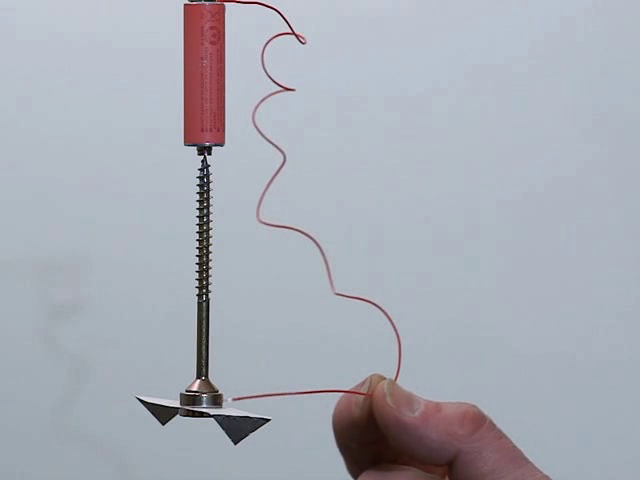
\includegraphics[height=0.4\textheight]{fig/lec03/homopolar_machine_video.png}}{fig/lec03/homopolar_machine_video.mp4}
            \vspace{0.75cm}
			\caption{Video of an operating homopolar machine (source: \href{https://de.wikipedia.org/wiki/Datei:Homopolarmotor_MAQ03891_smial_wp.ogv}{Wikimedia Commons}, Smial, \href{https://artlibre.org/licence/lal/en/}{Free Art License})}
		\end{subfigure}
		\hfill
		\begin{subfigure}[b]{0.49\textwidth}
			\centering
			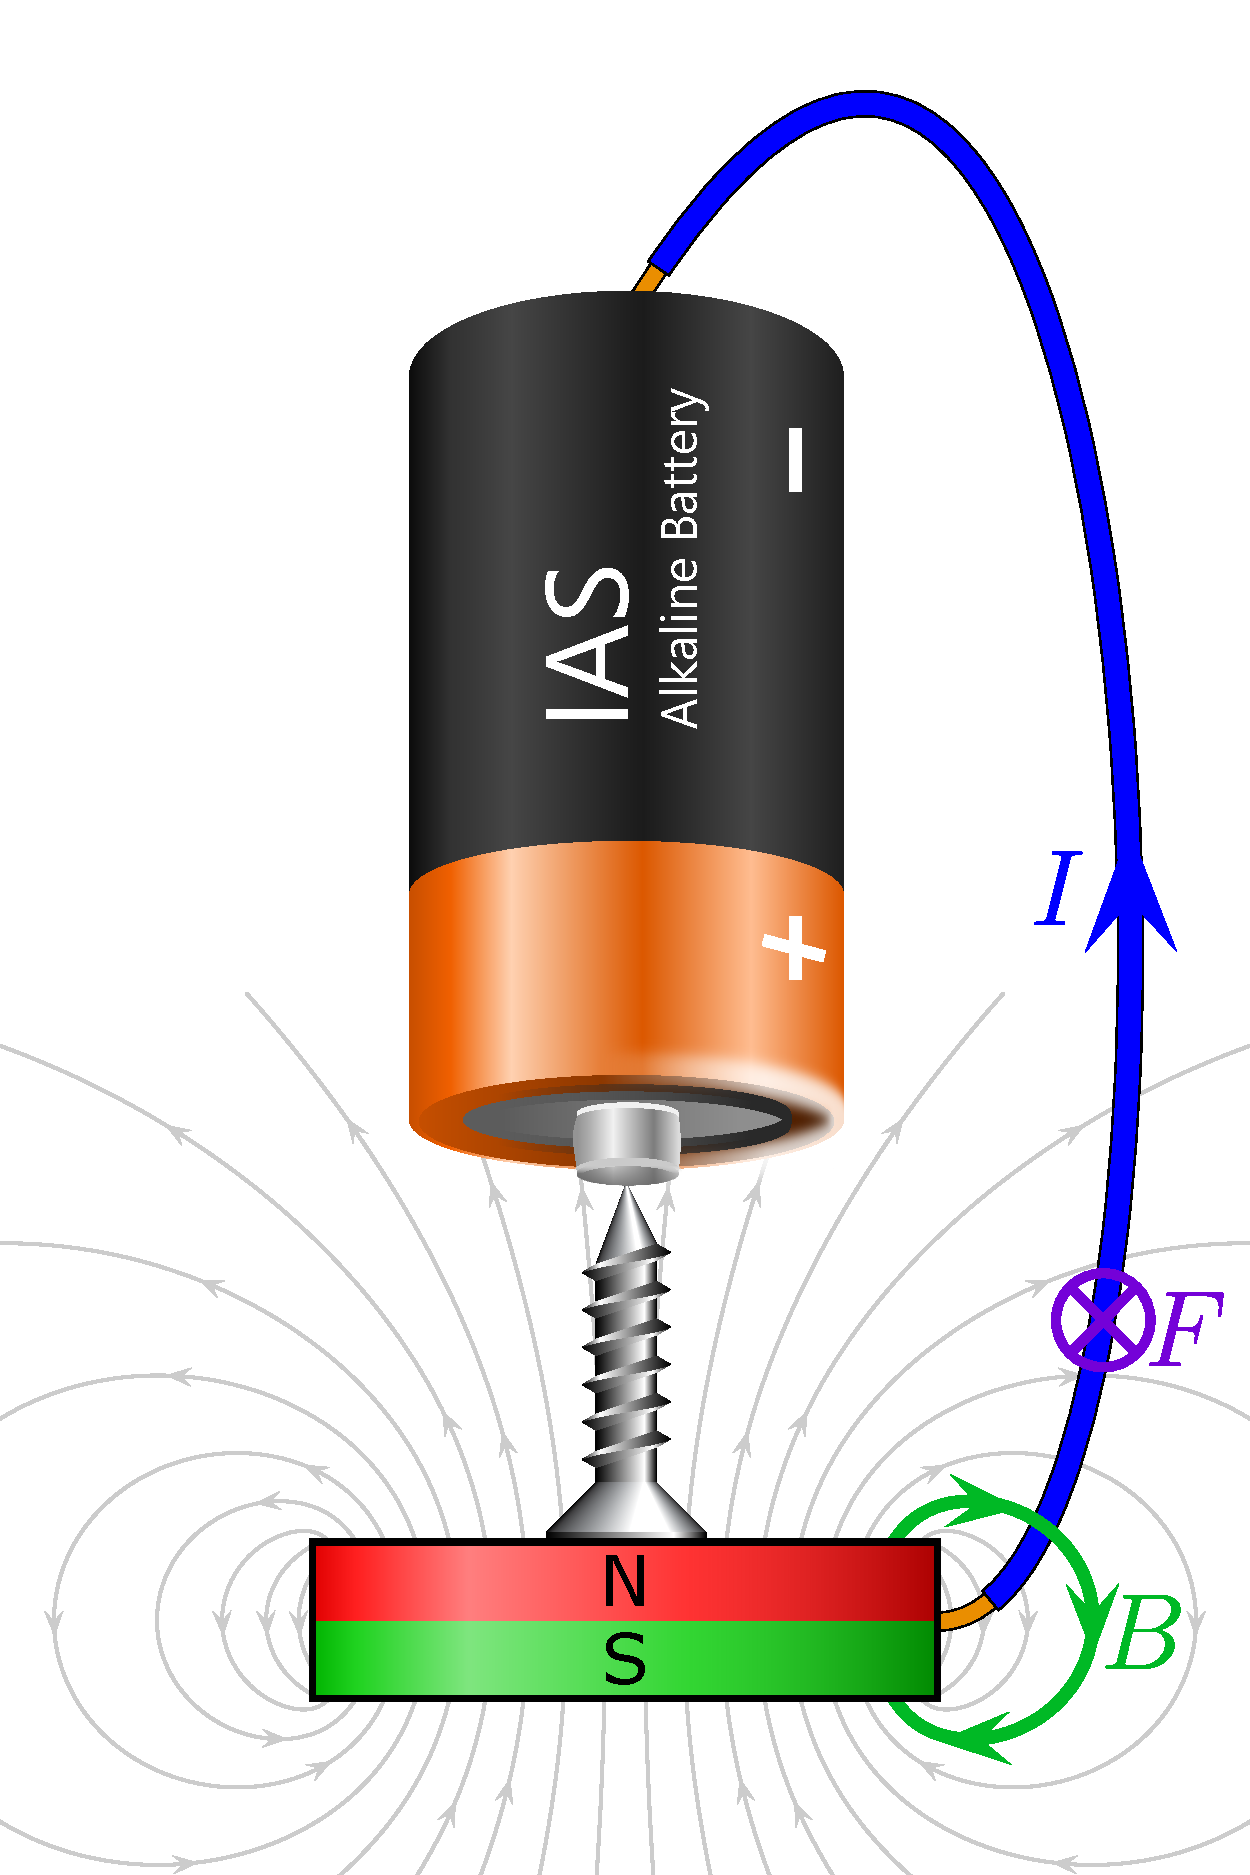
\includegraphics[width=0.47\textwidth]{fig/lec03/Homopolar_machine.pdf}
			\caption{Electric current, magnetic field and Lorentz force (adapted: \href{https://commons.wikimedia.org/wiki/File:Homopolar-motor.svg}{Wikimedia Commons}, M. Run, \href{https://creativecommons.org/licenses/by-sa/4.0/deed.en}{CC BY-SA})}
		\end{subfigure}
		\caption{Working principle of homopolar machines demonstrated with a simple permanent magnet, battery and screw design} 
        \label{fig:Homopolar_machine}
	\end{figure}
\end{frame}


%%%%%%%%%%%%%%%%%%%%%%%%%%%%%%%%%%%%%%%%%%%%%%%%%%%%%%%%%%%%%
%% Homopolar / unipolar machines (cont.) %%
%%%%%%%%%%%%%%%%%%%%%%%%%%%%%%%%%%%%%%%%%%%%%%%%%%%%%%%%%%%%%
\begin{frame}
	\frametitle{Homopolar / unipolar machines (cont.)}
    \begin{columns}
		\begin{column}{0.5\textwidth}
            \begin{itemize}
                \item  Homopolar machines are the simplest form of electric machines.
                \item They are also true DC machines, as the current and flux paths are unidirectional.
                \item<2-> The general design prevents connecting multiple rotor turns in series to increase the voltage, that is, only a relatively low voltage is induced.
                \item<3-> Consequently, homopolar machines require high currents (in the order of  \si{\kilo\ampere} or even \si{\mega\ampere}) to reach a useful power range which limited their application.
            \end{itemize}
		\end{column}
        \hfill
		\begin{column}{0.49\textwidth}
			\begin{figure}
				\centering
				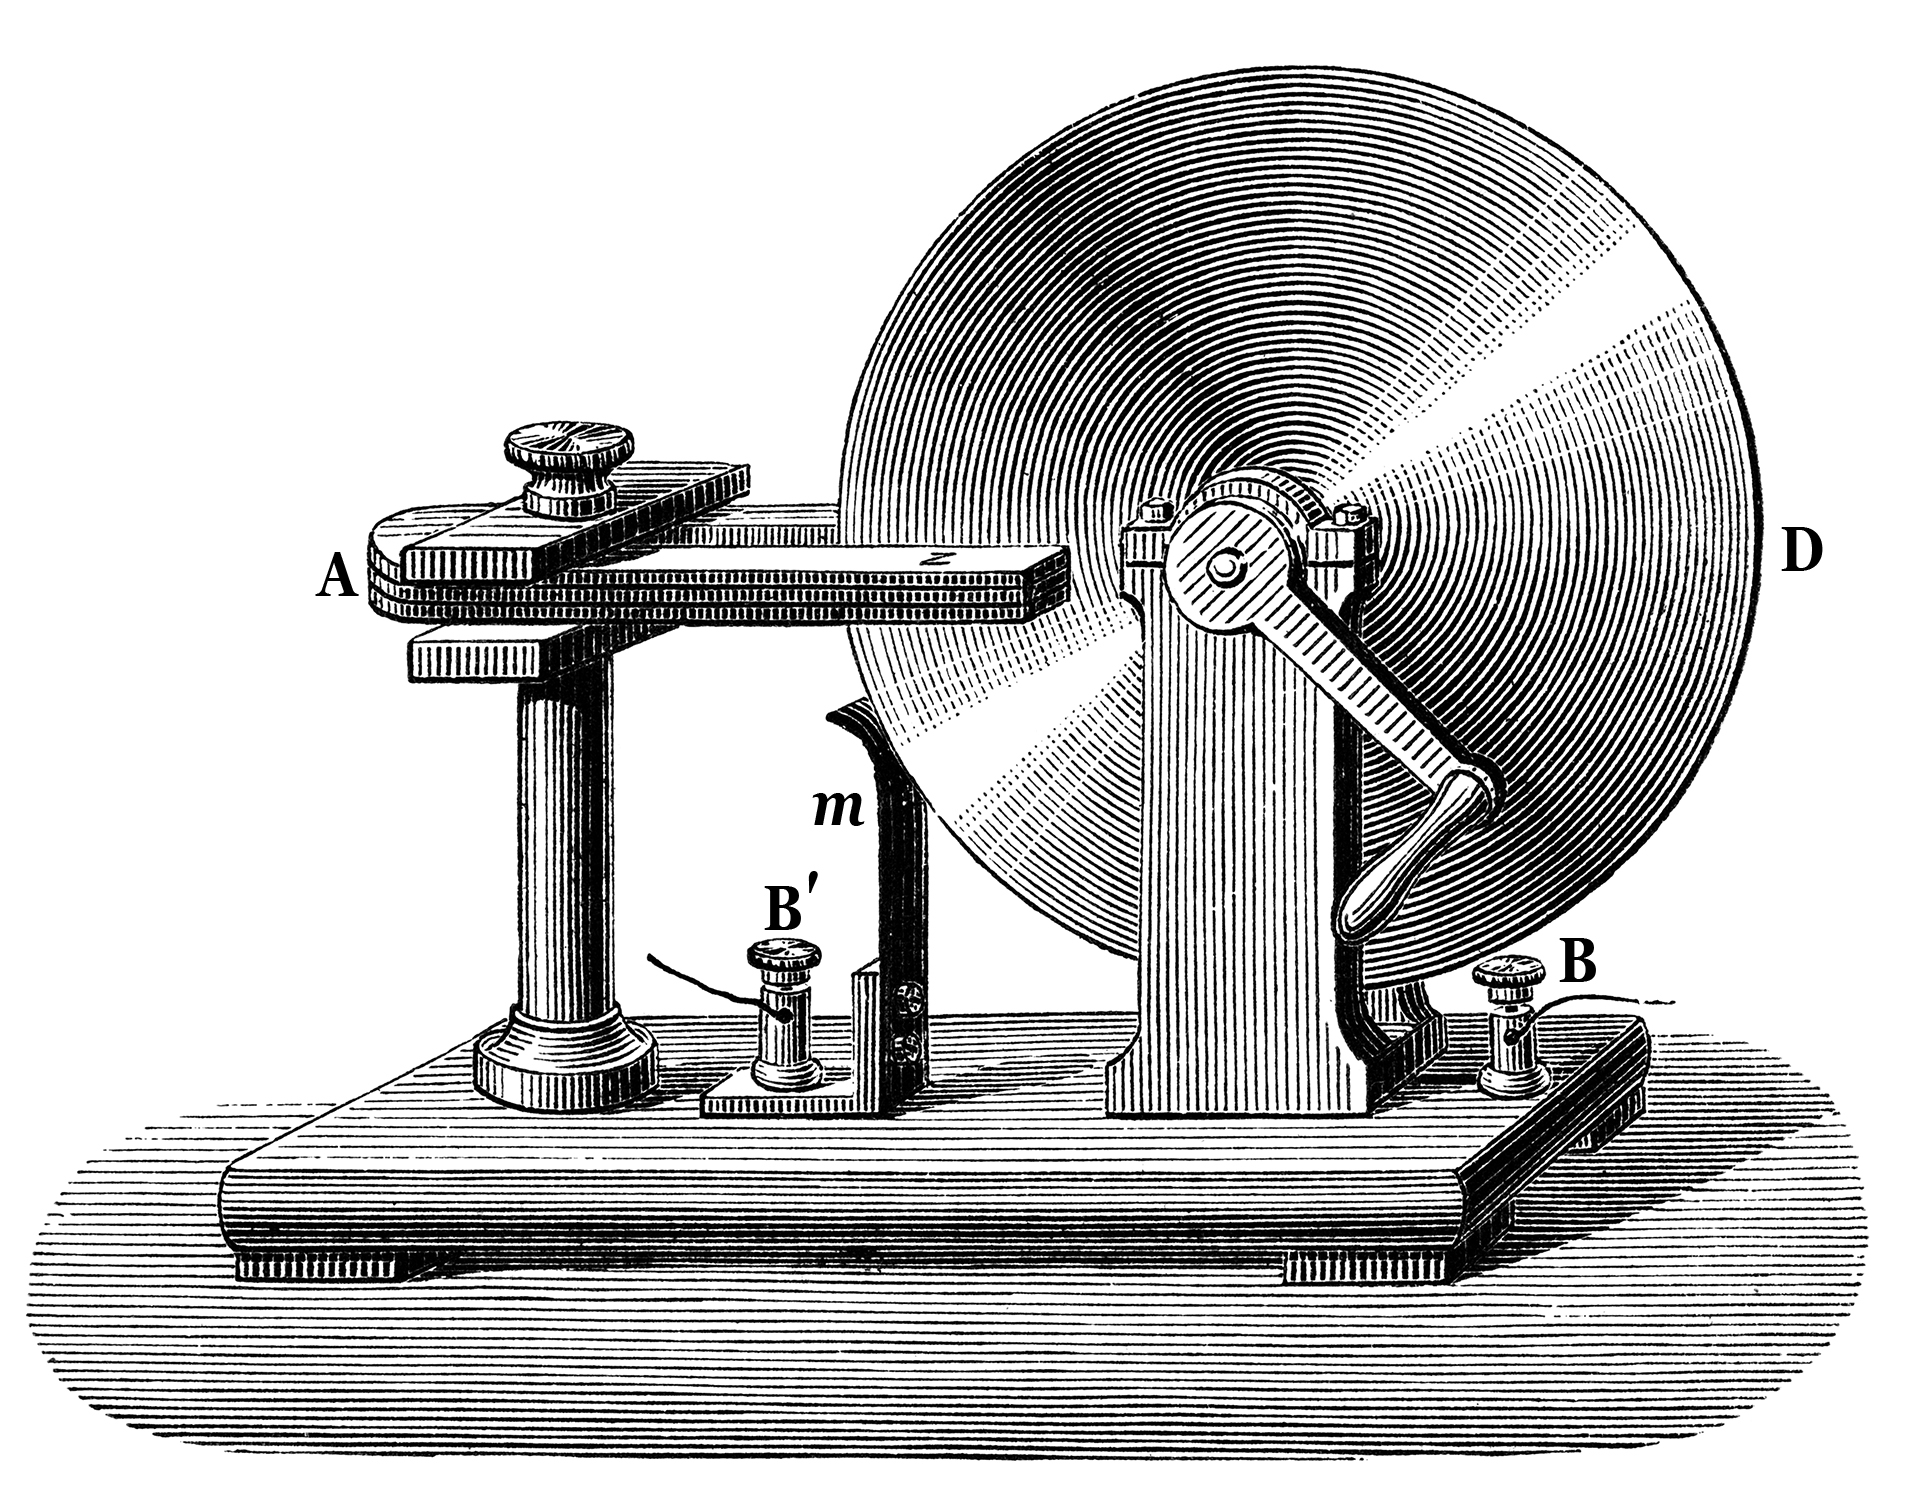
\includegraphics[width=0.8\textwidth]{fig/lec03/Faraday_disk_generator.jpg}
				\caption{The Faraday disk: another homopolar machine (source: \href{https://commons.wikimedia.org/wiki/File:Faraday_disk_generator.jpg}{Wikimedia Commons}, public domain)}
			\end{figure}
		\end{column}
		\end{columns}
\end{frame}

%%%%%%%%%%%%%%%%%%%%%%%%%%%%%%%%%%%%%%%%%%%%%%%%%%%%%%%%%%%%%
%% Working principle of usual DC machines %%
%%%%%%%%%%%%%%%%%%%%%%%%%%%%%%%%%%%%%%%%%%%%%%%%%%%%%%%%%%%%%
\begin{frame}
	\frametitle{Working principle of usual DC machines}
    \begin{columns}
		\begin{column}{0.5\textwidth}
            Let's consider \figref{fig:Simple_yoke_coil} and assume that the flux density $B$ is constant in the air gap and that the conductor loop has the axial length $l_\mathrm{z}$. \onslide<2->{According to the Lorentz force we have
			\begin{equation}
				F = I_\mathrm{a} B l_\mathrm{z} .
			\end{equation}}%  
			\onslide<3->{The torque $T$ on the conductor loop is given by
			\begin{equation}
				T = 2 F \frac{d}{2} \cos\left(\varepsilon\right) = I_\mathrm{a} B l_\mathrm{z} d \cos\left(\varepsilon\right).
			\end{equation}}%
			\onslide<4->{If the loop spins with an angular velocity $\omega$, mechanical power $P_\mathrm{me} = T\omega$ is transferred. 
			\\[1em]}%
			\onslide<5->{\textbf{Question:} What is happening if the coil is outside the magnetic field?}
		\end{column}
        \hfill
		\begin{column}{0.49\textwidth}
			\begin{figure}
				\centering
				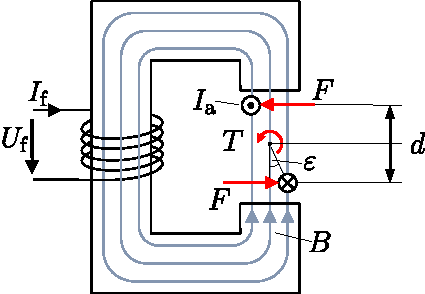
\includegraphics[width=0.9\textwidth]{fig/lec03/Simple_yoke_coil.pdf}
				\caption{Torque on a conductor loop (adapted from J.~B\"ocker, \textit{Elektrische Antriebstechnik}, Paderborn University, 2020)}
				\label{fig:Simple_yoke_coil}
			\end{figure}
		\end{column}
		\end{columns}
\end{frame}

%%%%%%%%%%%%%%%%%%%%%%%%%%%%%%%%%%%%%%%%%%%%%%%%%%%%%%%%%%%%%
%% DC-machine cross section %%
%%%%%%%%%%%%%%%%%%%%%%%%%%%%%%%%%%%%%%%%%%%%%%%%%%%%%%%%%%%%%
\begin{frame}
	\frametitle{DC-machine cross section}
    \begin{columns}
		\begin{column}{0.42\textwidth}
            \begin{itemize}
				\item To ensure a quasi-continous torque, the current through the conductor loop(s) in the rotor must have a constant direction.
				\item<2-> This is achieved by using a commutator (brushes).
				\item<3-> Compared to homopolar machines, DC machines require a mechanical rectification of the current.
			\end{itemize}
		\end{column}
        \hfill
		\begin{column}{0.55\textwidth}
			\begin{figure}
				\centering
				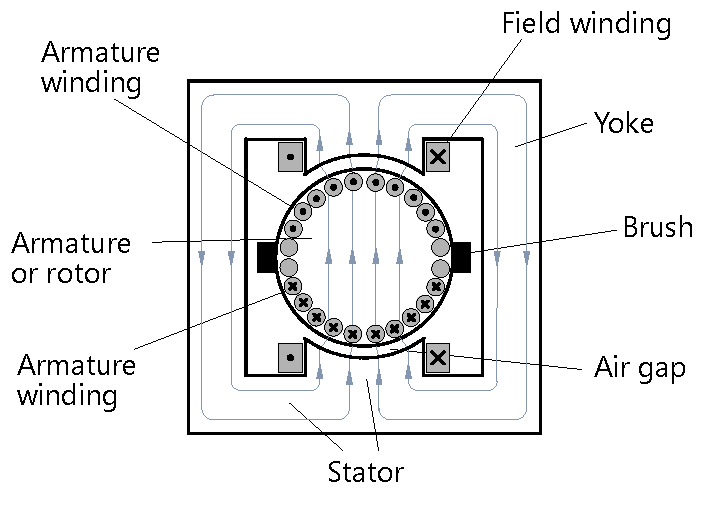
\includegraphics[width=0.925\textwidth]{fig/lec03/DC_machine_cross_section.pdf}
				\caption{Simplified DC machine cross section (adapted from J.~B\"ocker, \textit{Elektrische Antriebstechnik}, Paderborn University, 2020)}
				\label{fig:DC_machine_cross_section}
			\end{figure}
		\end{column}
		\end{columns}
\end{frame}

%%%%%%%%%%%%%%%%%%%%%%%%%%%%%%%%%%%%%%%%%%%%%%%%%%%%%%%%%%%%%
%% Commutation %%
%%%%%%%%%%%%%%%%%%%%%%%%%%%%%%%%%%%%%%%%%%%%%%%%%%%%%%%%%%%%%
\begin{frame}
	\frametitle{Commutation}
    \begin{figure}
		\centering
		\movie{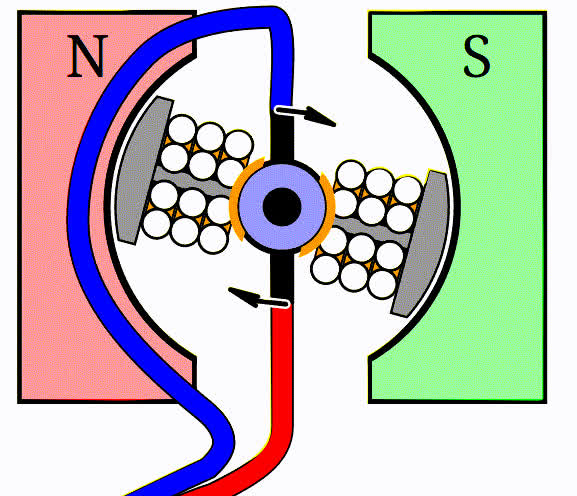
\includegraphics[height=0.65\textheight]{fig/lec03/DC_machine_simple_animation.jpeg}}{fig/lec03/DC_machine_simple_animation.gif}
		\caption{Animation of the commutation process \\(source: \href{https://commons.wikimedia.org/wiki/File:Animation_einer_Gleichstrommaschine_(Variante-Langsam).gif}{Wikimedia Commons}, M. Frey, \href{https://creativecommons.org/licenses/by-sa/3.0/deed.en}{CC BY-SA 3.0})}
	\end{figure}
\end{frame}

%%%%%%%%%%%%%%%%%%%%%%%%%%%%%%%%%%%%%%%%%%%%%%%%%%%%%%%%%%%%%
%% Armature and commutator %%
%%%%%%%%%%%%%%%%%%%%%%%%%%%%%%%%%%%%%%%%%%%%%%%%%%%%%%%%%%%%%
\begin{frame}
	\frametitle{Armature and commutator}
    \begin{figure}
		\centering
		\begin{subfigure}[b]{0.49\textwidth}
			\centering
			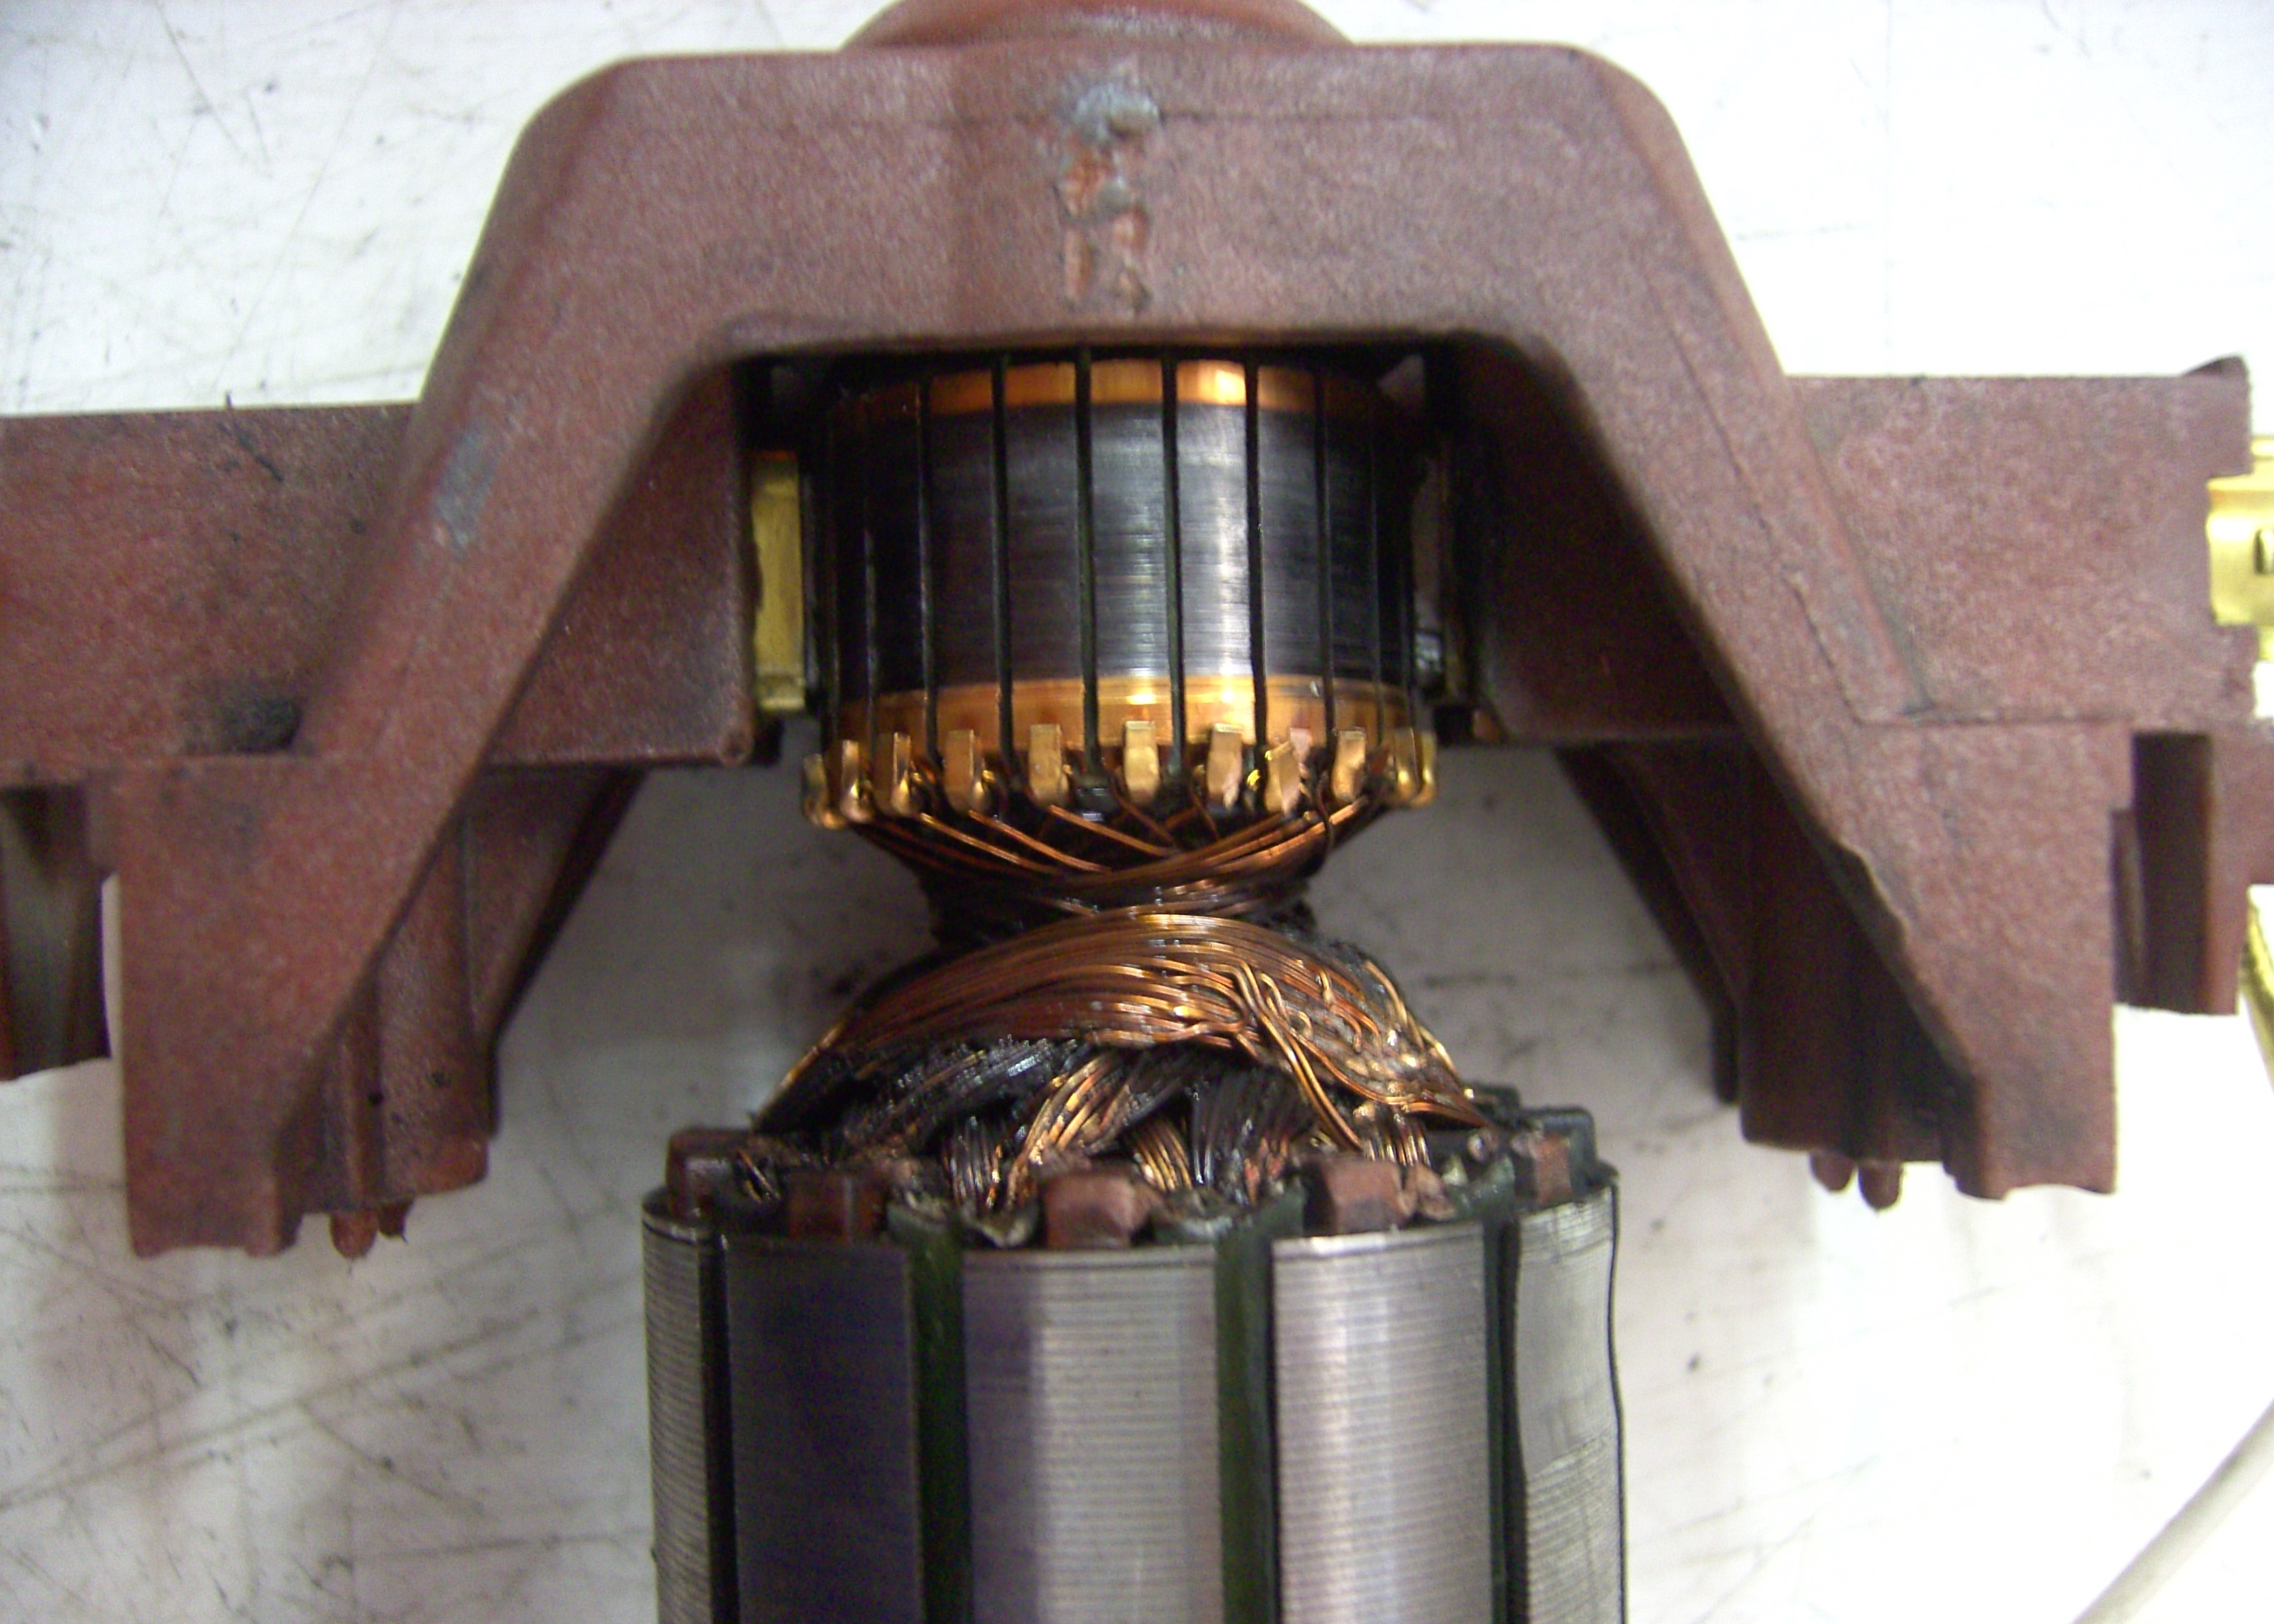
\includegraphics[width=0.85\textwidth]{fig/lec03/Commutator_Universalmachine.jpg}
			\caption{Commutator with brushes and springs (source: \href{https://commons.wikimedia.org/wiki/File:Kommutator_eines_Universalmotor.JPGg}{Wikimedia Commons}, Marrrci, \href{https://creativecommons.org/licenses/by-sa/3.0/deed.en}{CC BY-SA 3.0})}
		\end{subfigure}
		\hfill
		\begin{subfigure}[b]{0.49\textwidth}
			\centering
			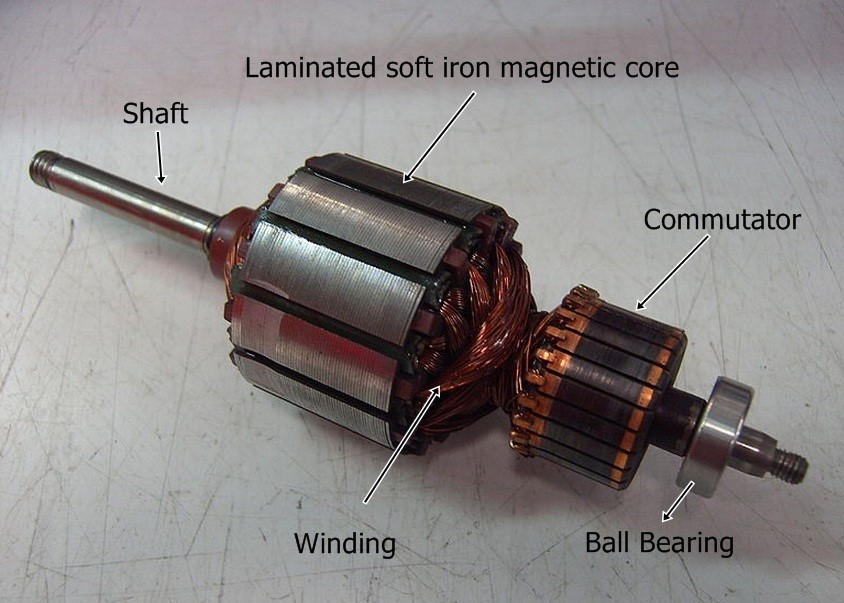
\includegraphics[width=0.85\textwidth]{fig/lec03/DC_armature_example.jpg}
			\caption{DC machine armature with commutator (source: \href{https://commons.wikimedia.org/wiki/File:Motor_rotor.jpg}{Wikimedia Commons}, public domain)}
		\end{subfigure}
		\caption{Examples of commutators and armatures} 
        \label{fig:Armature_and_commutator}
	\end{figure}
\end{frame}

%%%%%%%%%%%%%%%%%%%%%%%%%%%%%%%%%%%%%%%%%%%%%%%%%%%%%%%%%%%%%
%% Armature and commutator (cont.) %%
%%%%%%%%%%%%%%%%%%%%%%%%%%%%%%%%%%%%%%%%%%%%%%%%%%%%%%%%%%%%%
\begin{frame}
	\frametitle{Armature and commutator (cont.)}
    \begin{figure}
		\ContinuedFloat
		\centering
		\begin{subfigure}[b]{0.49\textwidth}
			\centering
			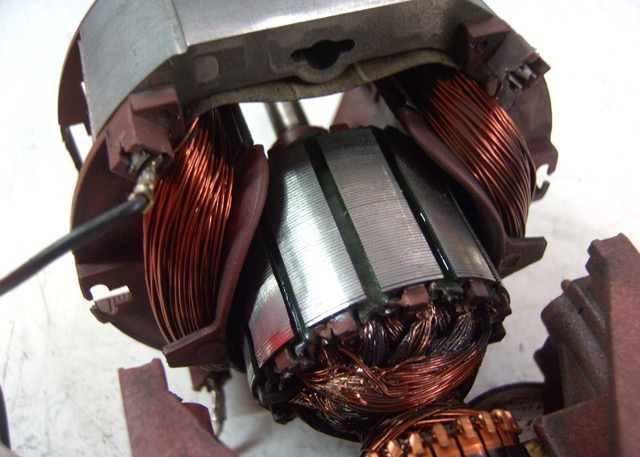
\includegraphics[width=0.85\textwidth]{fig/lec03/Stator_Rotor_Universalmachine.jpg}
			\caption{Armature inside stator (source: \href{https://commons.wikimedia.org/wiki/File:Universalmotor_1.JPG}{Wikimedia Commons}, Marrrci, \href{https://creativecommons.org/licenses/by-sa/3.0/deed.en}{CC BY-SA 3.0})}
		\end{subfigure}
		\hfill
		\begin{subfigure}[b]{0.49\textwidth}
			\centering
			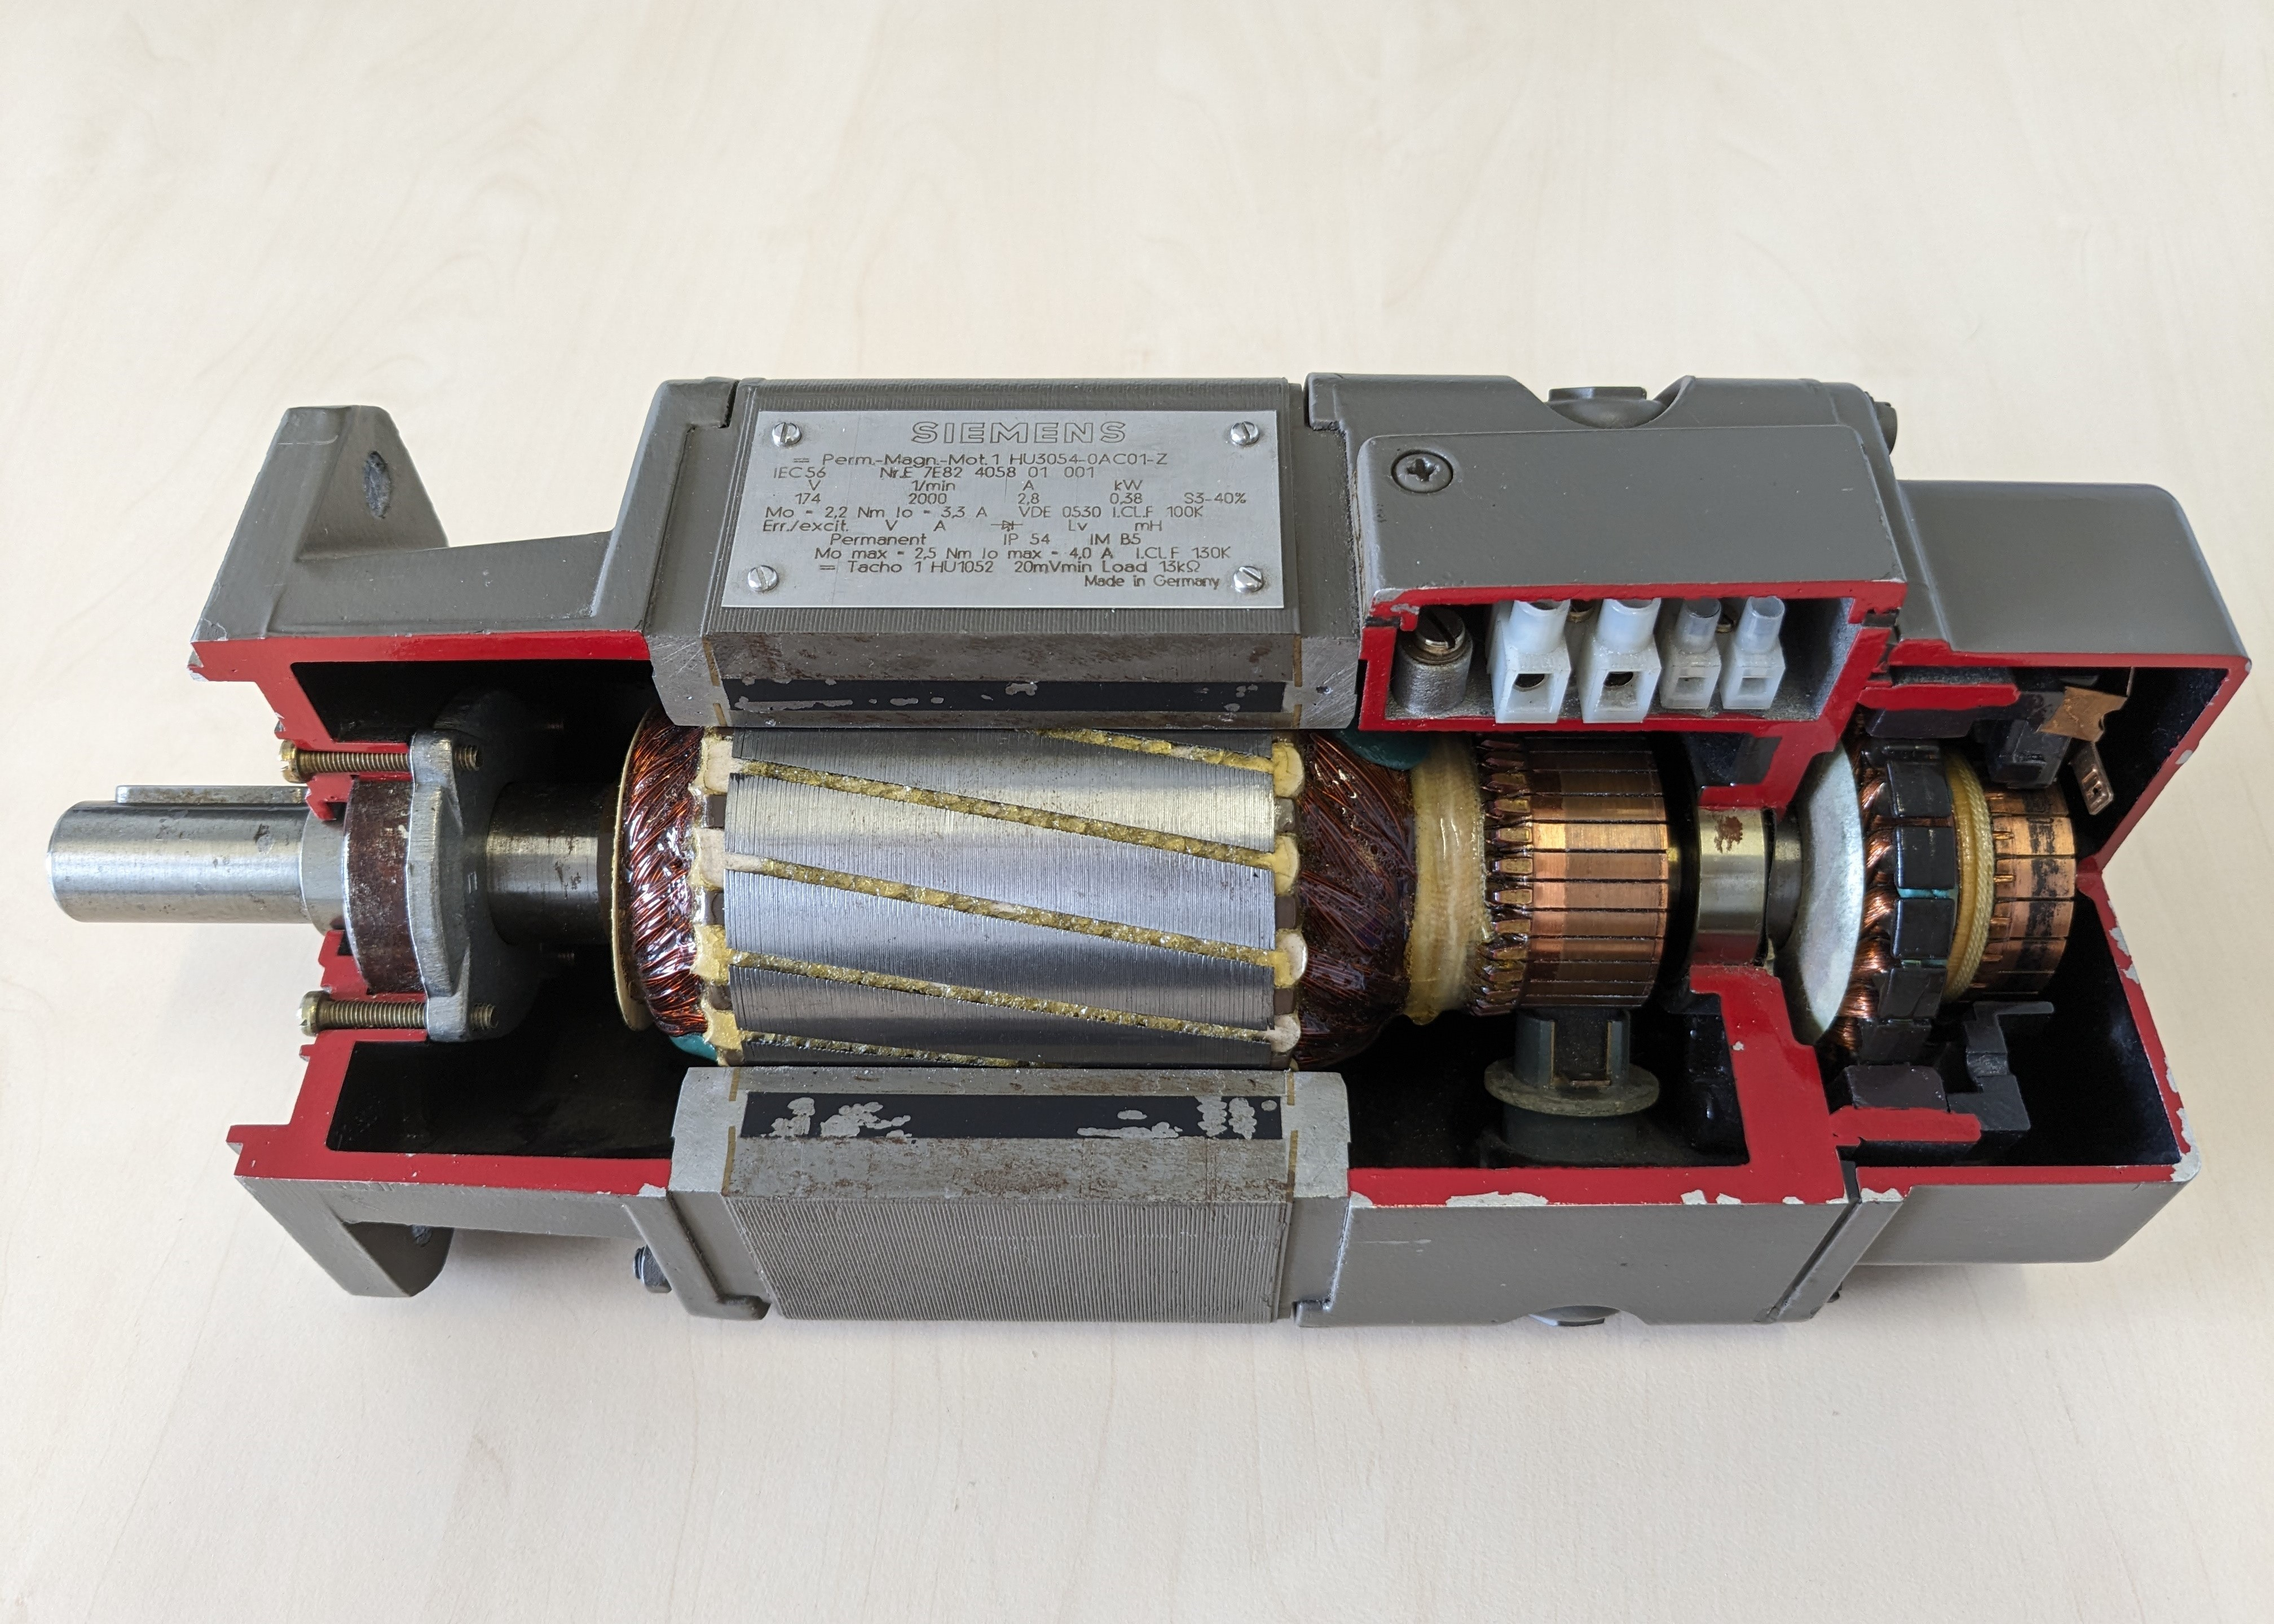
\includegraphics[width=0.85\textwidth]{fig/lec03/DC_Machine_PM.jpg}
			\caption{DC machine with permanent magnet excitation and tacho speed sensor}
		\end{subfigure}
		\caption{Examples of commutators and armatures (cont.)} 
        \label{fig:Armature_and_commutator_02}
	\end{figure}
\end{frame}

%%%%%%%%%%%%%%%%%%%%%%%%%%%%%%%%%%%%%%%%%%%%%%%%%%%%%%%%%%%%%
%% Basic structure of the armature %%
%%%%%%%%%%%%%%%%%%%%%%%%%%%%%%%%%%%%%%%%%%%%%%%%%%%%%%%%%%%%%
\begin{frame}
	\frametitle{Basic structure of the armature}
    \begin{figure}
        \centering
        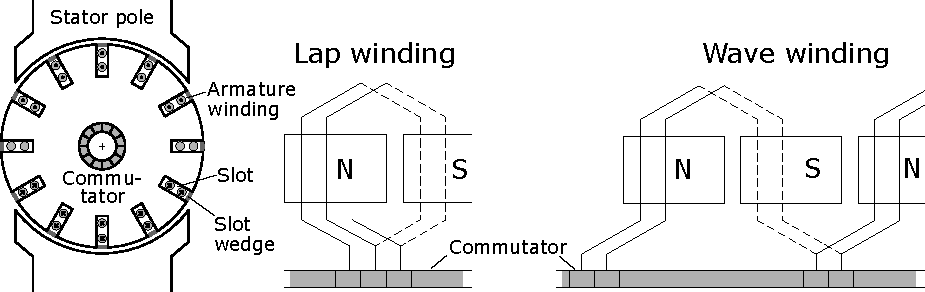
\includegraphics[width=0.925\textwidth]{fig/lec03/Armature_slots.pdf}
        \caption{Cross section of a drum-type armature including principle winding schemes (adapted from W.~Novender, \textit{Elektrische Maschinen}, Technische Hochschule Mittelhessen, 2023)}
    \end{figure}
\end{frame}

%%%%%%%%%%%%%%%%%%%%%%%%%%%%%%%%%%%%%%%%%%%%%%%%%%%%%%%%%%%%%
%% Winding wiring types %%
%%%%%%%%%%%%%%%%%%%%%%%%%%%%%%%%%%%%%%%%%%%%%%%%%%%%%%%%%%%%%
\begin{frame}
	\frametitle{Types of winding conductors}
    \begin{figure}
        \centering
        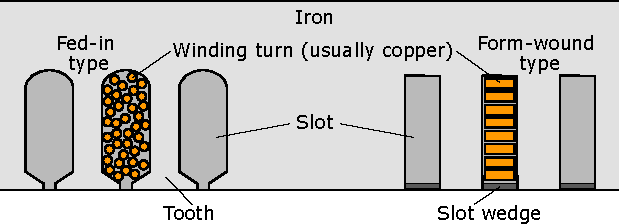
\includegraphics[width=0.8\textwidth]{fig/lec03/Winding_turn_types.pdf}
        \caption{Types of winding conductors -- unwound representation along the circumference (adapted from J.~B\"ocker, \textit{Controlled Three-Phase Drives}, Paderborn University, 2021)}
    \end{figure}
\end{frame}

%%%%%%%%%%%%%%%%%%%%%%%%%%%%%%%%%%%%%%%%%%%%%%%%%%%%%%%%%%%%%
%% Commutation process with an armature lap winding %%
%%%%%%%%%%%%%%%%%%%%%%%%%%%%%%%%%%%%%%%%%%%%%%%%%%%%%%%%%%%%%
\begin{frame}
	\frametitle{Commutation process with an armature lap winding}
	\vspace{-0.1cm}
    \begin{figure}
        \centering
        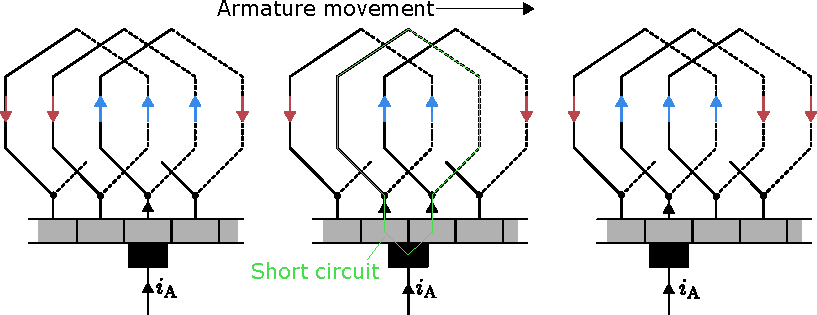
\includegraphics[height=0.6\textheight]{fig/lec03/Commutation_process_lap_winding.pdf}
        \caption{Three still images of the commutation process with a simplified winding representation (from left to right): when the brush touches two commutator segments, the according conductor loop is short-circuited and the current is reduced to zero. The brush then moves to the next commutator segment and the current starts flowing again but in the opposite direction (adapted from W.~Novender, \textit{Elektrische Maschinen}, Technische Hochschule Mittelhessen, 2023).}
    \end{figure}
\end{frame}

%%%%%%%%%%%%%%%%%%%%%%%%%%%%%%%%%%%%%%%%%%%%%%%%%%%%%%%%%%%%%
%% DC machines with multiple pole pairs %%
%%%%%%%%%%%%%%%%%%%%%%%%%%%%%%%%%%%%%%%%%%%%%%%%%%%%%%%%%%%%%
\begin{frame}
	\frametitle{DC machines with multiple pole pairs}
    \begin{columns}
		\begin{column}{0.42\textwidth}
            \begin{itemize}
				\item To reduce the effective length per armature conductor loop, the winding can form multiple pole pairs $p$.
				\item<2-> This will reduce the inductance per loop which is beneficial for the commutation process.
				\item<3-> The stator excitation must meet the same number of pole pairs.
				\item<4-> Given some inner stator diameter $d_\mathrm{s}$, the resulting pole pitch is:
			\end{itemize}
			\onslide<4->{\begin{equation}
				\tau_\mathrm{p} = \frac{\pi d_\mathrm{s}}{2p}, \quad \rho_\mathrm{p} = \frac{\pi}{p} .
			\end{equation}}%
		\end{column}
        \hfill
		\begin{column}{0.55\textwidth}
			\begin{figure}
				\centering
				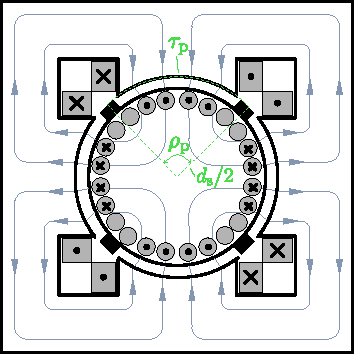
\includegraphics[width=0.64\textwidth]{fig/lec03/DC_machine_cross_section_two_pole_pairs.pdf}
				\caption{Simplified DC machine cross section with $p=2$ pole pairs (adapted from J.~B\"ocker, \textit{Elektrische Antriebstechnik}, Paderborn University, 2020)}
				\label{fig:DC_machine_cross_section_two_pole_pairs}
			\end{figure}
		\end{column}
		\end{columns}
\end{frame}

%%%%%%%%%%%%%%%%%%%%%%%%%%%%%%%%%%%%%%%%%%%%%%%%%%%%%%%%%%%%%
%% Winding characteristics (cont.) %%
%%%%%%%%%%%%%%%%%%%%%%%%%%%%%%%%%%%%%%%%%%%%%%%%%%%%%%%%%%%%%
\begin{frame}
	\frametitle{Armature winding characteristics}
	For describing the armature winding layout, the following parameters are introduced:
	\begin{gather*}
		Q: \mbox{number of slots}, \quad N_\mathrm{c}: \mbox{number of conductor turns per coil}, \\ K: \mbox{number of commutator elements}, \quad u = K/Q: \mbox{slot to commutator ratio}, \\z_\mathrm{a} = 2 K N_\mathrm{c}: \mbox{total number of armature conductors}.
	\end{gather*}
    \begin{figure}
        \centering
        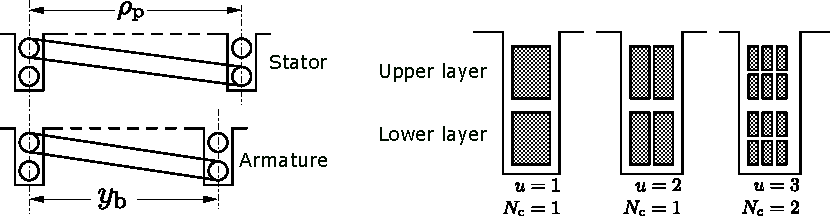
\includegraphics[height=0.35\textheight]{fig/lec03/Lap_winding_characteristics.pdf}
        \caption{Coil width and slot design characteristics (adapted from W.~Novender, \textit{Elektrische Maschinen}, Technische Hochschule Mittelhessen, 2023)}
		\label{fig:Lap_winding_characteristics}
    \end{figure}
\end{frame}

%%%%%%%%%%%%%%%%%%%%%%%%%%%%%%%%%%%%%%%%%%%%%%%%%%%%%%%%%%%%%
%% Double layer winding %%
%%%%%%%%%%%%%%%%%%%%%%%%%%%%%%%%%%%%%%%%%%%%%%%%%%%%%%%%%%%%%
\begin{frame}
	\frametitle{Double layer winding}
	\begin{itemize}
		\item The forward conductor of one coil and the return conductor of another coil are placed in the same slot. This is the common winding scheme (although not limited to it).
		\item Enables chording of the winding ($\rho_\mathrm{p}\neq y_\mathrm{b}$), another degree of freedom for the machine design (cf. \figref{fig:Lap_winding_characteristics}).
	\end{itemize}
    \begin{figure}
        \centering
        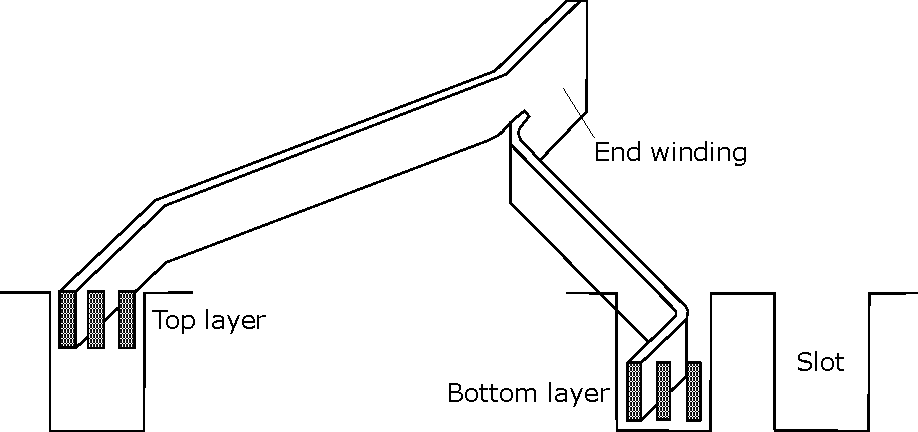
\includegraphics[height=0.45\textheight]{fig/lec03/Double_layer_winding.pdf}
        \caption{Double layer winding with $u=3$ with a solid conductor element (which can be pre-manufactured for cost reasons -- inspired from A. Binder, \textit{Elektrische Maschinen und Antriebe}, Vol. 2, Springer, 2017)}
    \end{figure}
\end{frame}

%%%%%%%%%%%%%%%%%%%%%%%%%%%%%%%%%%%%%%%%%%%%%%%%%%%%%%%%%%%%%
%% Lap winding characteristics %%
%%%%%%%%%%%%%%%%%%%%%%%%%%%%%%%%%%%%%%%%%%%%%%%%%%%%%%%%%%%%%
\begin{frame}
	\frametitle{Lap winding characteristics}
    \begin{columns}
		\begin{column}{0.42\textwidth}
            \begin{itemize}
				\item Back pitch $y_\mathrm{b}$: coil span from the back end
				\item<2-> Front pitch $y_\mathrm{f}$: coil span from the front end
				\item<3-> Resultant pitch $y_\mathrm{r}$: distance between two consecutive coils
				\item<4-> Commutator pitch $y_\mathrm{c}$: distance between two consecutive commutator segments
			\end{itemize}
			\vspace{-0.4cm}
			\onslide<5->{\begin{varblock}{Progressive winding}
				\figref{fig:Lap_winding_distances} shows a progressive winding layout with $y_\mathrm{b} > y_\mathrm{f}$, i.e., the coils do not cross themselves.
			\end{varblock}}%
		\end{column}
        \hfill
		\begin{column}{0.55\textwidth}
			\begin{figure}
				\centering
				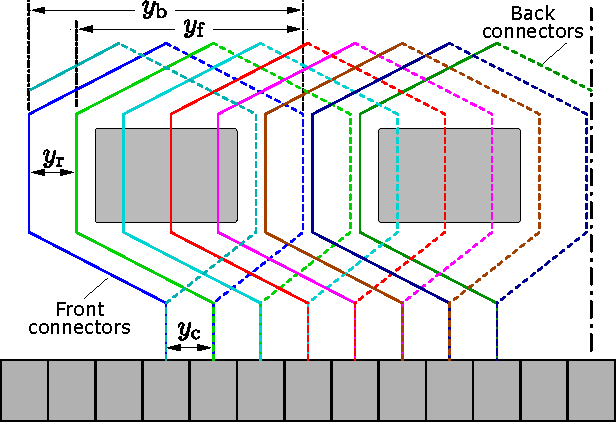
\includegraphics[width=0.85\textwidth]{fig/lec03/Lap_winding_distances.pdf}
				\caption{Distance definitions of the armature lap winding (adapted from W.~Novender, \textit{Elektrische Maschinen}, Technische Hochschule Mittelhessen, 2023)}
				\label{fig:Lap_winding_distances}
			\end{figure}
		\end{column}
		\end{columns}
\end{frame}

%%%%%%%%%%%%%%%%%%%%%%%%%%%%%%%%%%%%%%%%%%%%%%%%%%%%%%%%%%%%%
%% Lap winding characteristics (cont.) %%
%%%%%%%%%%%%%%%%%%%%%%%%%%%%%%%%%%%%%%%%%%%%%%%%%%%%%%%%%%%%%
\begin{frame}
	\frametitle{Lap winding characteristics (cont.)}
    \begin{columns}
		\begin{column}{0.42\textwidth}
			\begin{varblock}{Retrogressive winding}
				\figref{fig:Lap_winding_distances_retrogressive} shows a Retrogressive winding layout with $y_\mathrm{b} < y_\mathrm{f}$, i.e., each coil crosses itself.
			\end{varblock}
			\begin{itemize}
				\item<2-> Retrogressive windings require more conductor material due to the crossing of the coils and, therefore, are less common.
				\item<3-> Technical feasibility requires $y_\mathrm{b} - y_\mathrm{f} = \pm y_\mathrm{c}$, i.e., the lap winding progresses or retrogresses by one commutator element.
			\end{itemize}
		\end{column}
        \hfill
		\begin{column}{0.55\textwidth}
			\begin{figure}
				\centering
				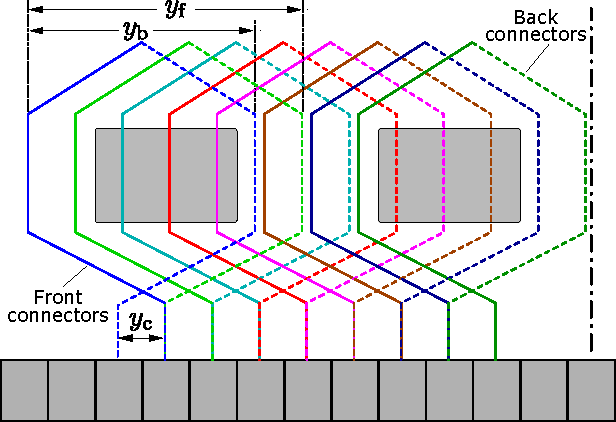
\includegraphics[width=0.85\textwidth]{fig/lec03/Lap_winding_distances_retrogressive.pdf}
				\caption{Lap winding with a retrogressive scheme (adapted from W.~Novender, \textit{Elektrische Maschinen}, Technische Hochschule Mittelhessen, 2023)}
				\label{fig:Lap_winding_distances_retrogressive}
			\end{figure}
		\end{column}
		\end{columns}
\end{frame}


%%%%%%%%%%%%%%%%%%%%%%%%%%%%%%%%%%%%%%%%%%%%%%%%%%%%%%%%%%%%%
%% Lap winding %%
%%%%%%%%%%%%%%%%%%%%%%%%%%%%%%%%%%%%%%%%%%%%%%%%%%%%%%%%%%%%%
\begin{frame}
	\frametitle{Lap winding: final remarks and single pole pair example}
	\begin{columns}
		\begin{column}{0.35\textwidth}
			\begin{itemize}
				\item Armature turns per pole: $N_\mathrm{p} = \frac{KN_\mathrm{c}}{2p}$
				\item Current per armature conductor: $I_\mathrm{c} = \frac{I_\mathrm{a}}{2 p}$
			\end{itemize}
			\onslide<2->{\begin{varblock}{Parallel connection of poles}
				For $p>1$ the lap winding parallels the armature coils for each pole enabling a higher current (but limited voltage) rating.
			\end{varblock}}%
		\end{column}
		\hfill
		\begin{column}{0.65\textwidth}
			\begin{figure}
				\centering
				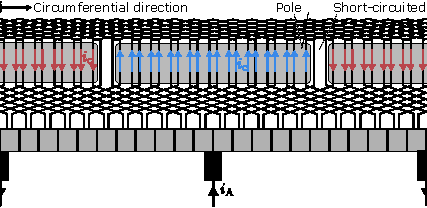
\includegraphics[width=0.95\textwidth]{fig/lec03/Lap_winding.pdf}
				\caption{Lap winding with commutator unrolled along the circumferential coordinate}
			\end{figure}
		\end{column}
	\end{columns}
\end{frame}

%%%%%%%%%%%%%%%%%%%%%%%%%%%%%%%%%%%%%%%%%%%%%%%%%%%%%%%%%%%%%
%% Wave winding characteristics %%
%%%%%%%%%%%%%%%%%%%%%%%%%%%%%%%%%%%%%%%%%%%%%%%%%%%%%%%%%%%%%
\begin{frame}
	\frametitle{Wave winding characteristics}
    \begin{columns}
		\begin{column}{0.42\textwidth}
            \begin{itemize}
				\item Commutator pitch (wave winding): $y_\mathrm{c} = y_\mathrm{f} + y_\mathrm{b}$, i.e., each coil spans (nearly) the entire pole pitch.  
			\end{itemize}
			\vspace{-0.4cm}
			\onslide<2->{\begin{varblock}{Progressive winding}
				\figref{fig:Wave_winding_distances} shows a progressive winding layout since each new wave winding coil starts one commutator element to the right. 
			\end{varblock}}
		\end{column}
        \hfill
		\begin{column}{0.55\textwidth}
			\begin{figure}
				\centering
				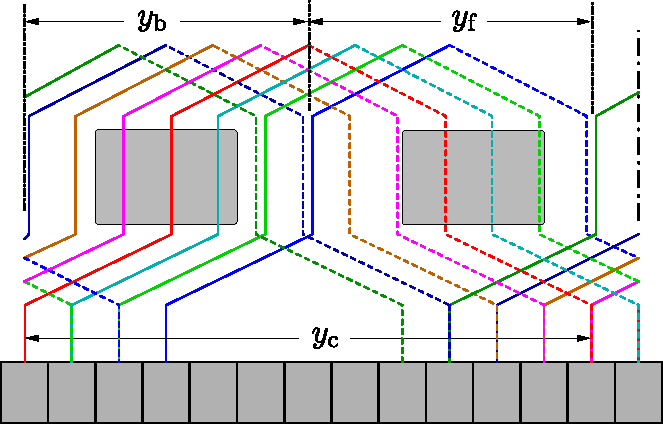
\includegraphics[width=0.85\textwidth]{fig/lec03/Wave_winding_distances.pdf}
				\caption{Distance definitions of the armature wave winding (adapted from W.~Novender, \textit{Elektrische Maschinen}, Technische Hochschule Mittelhessen, 2023)}
				\label{fig:Wave_winding_distances}
			\end{figure}
		\end{column}
		\end{columns}
\end{frame}

%%%%%%%%%%%%%%%%%%%%%%%%%%%%%%%%%%%%%%%%%%%%%%%%%%%%%%%%%%%%%
%% Wave winding %%
%%%%%%%%%%%%%%%%%%%%%%%%%%%%%%%%%%%%%%%%%%%%%%%%%%%%%%%%%%%%%
\begin{frame}
	\frametitle{Wave winding: final remarks and single pole pair example}
	\begin{columns}
		\begin{column}{0.35\textwidth}
			\begin{itemize}
				\item Armature turns per pole: $N_\mathrm{p} = \frac{K N_\mathrm{c}}{2}$
				\item Current per armature conductor: $I_\mathrm{c} = \frac{I_\mathrm{a}}{2}$
			\end{itemize}
			\onslide<2->{\begin{varblock}{Series connection of poles}
				For $p>1$ the wave winding connects the armature coils for all poles in series enabling a higher voltage (but limited current) rating.
			\end{varblock}}
		\end{column}
		\hfill
		\begin{column}{0.65\textwidth}
			\begin{figure}
				\centering
				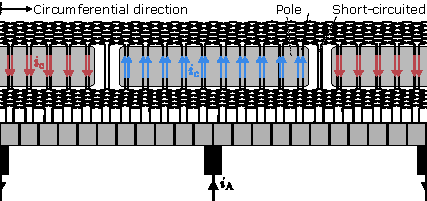
\includegraphics[width=0.95\textwidth]{fig/lec03/Wave_winding.pdf}
				\caption{Wave winding with commutator unrolled along the circumferential coordinate}
			\end{figure}
		\end{column}
	\end{columns}
\end{frame}

%%%%%%%%%%%%%%%%%%%%%%%%%%%%%%%%%%%%%%%%%%%%%%%%%%%%%%%%%%%%%
%% Lap and wave winding comparison %%
%%%%%%%%%%%%%%%%%%%%%%%%%%%%%%%%%%%%%%%%%%%%%%%%%%%%%%%%%%%%%
\begin{frame}
	\frametitle{Lap and wave winding comparison}
	Introducing the parameter 
	\begin{equation}
		a = \mbox{number of parallel armature conductors}
		\label{eq:Parallel_conductors}
	\end{equation}
	we can wrap up the following summary:\pause
	\begin{equation}
		\mbox{Current per conductor: } I_\mathrm{c} = \frac{I_\mathrm{a}}{2 a}, \quad \mbox{Armature turns per pole: } N_\mathrm{p} = \frac{K N_\mathrm{c}}{2 a}.
	\end{equation}\pause
	\begin{varblock}{Comparison}
		\begin{itemize}
			\item Lap winding: $a = p$ (parallel connection of poles)
			\item Wave winding: $a = 1$ (series connection of poles)
		\end{itemize}
	\end{varblock}
\end{frame}

%%%%%%%%%%%%%%%%%%%%%%%%%%%%%%%%%%%%%%%%%%%%%%%%%%%%%%%%%%%%%
%% Commutation process %%
%%%%%%%%%%%%%%%%%%%%%%%%%%%%%%%%%%%%%%%%%%%%%%%%%%%%%%%%%%%%%
\begin{frame}
	\frametitle{Commutation process}
	During the commutation time $\Delta t_\mathrm{c}$ the brush bridges two commutator segments and the short-circuited conductor coil current $i_\mathrm{c}$ is changing signs.\onslide<2->{ Here, two major scenarios can be distinguished:}
	\begin{itemize}
		\item<2-> The commutation is such fast that high local current densities are prevented.
		\item<3-> The commutation is slow and high local current densities lead to sparking effects.
	\end{itemize}
    \begin{figure}
        \centering
        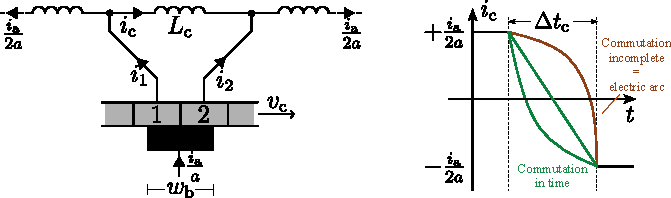
\includegraphics[width=0.75\textwidth]{fig/lec03/Commutation_process_time_trajectory.pdf}
        \caption{Left: simplified equivalent circuit diagram of the short-circuited coil during commutation. Right: qualitative trajectories of the conductor current $i_\mathrm{c}$} 
		\label{fig:Commutation_process_time_trajectory}
    \end{figure}
\end{frame}

%%%%%%%%%%%%%%%%%%%%%%%%%%%%%%%%%%%%%%%%%%%%%%%%%%%%%%%%%%%%%
%% Commutation process %%
%%%%%%%%%%%%%%%%%%%%%%%%%%%%%%%%%%%%%%%%%%%%%%%%%%%%%%%%%%%%%
\begin{frame}
	\frametitle{Commutation process (cont.)}
	\begin{columns}
		\begin{column}{0.4\textwidth}
			\begin{figure}
				\centering
				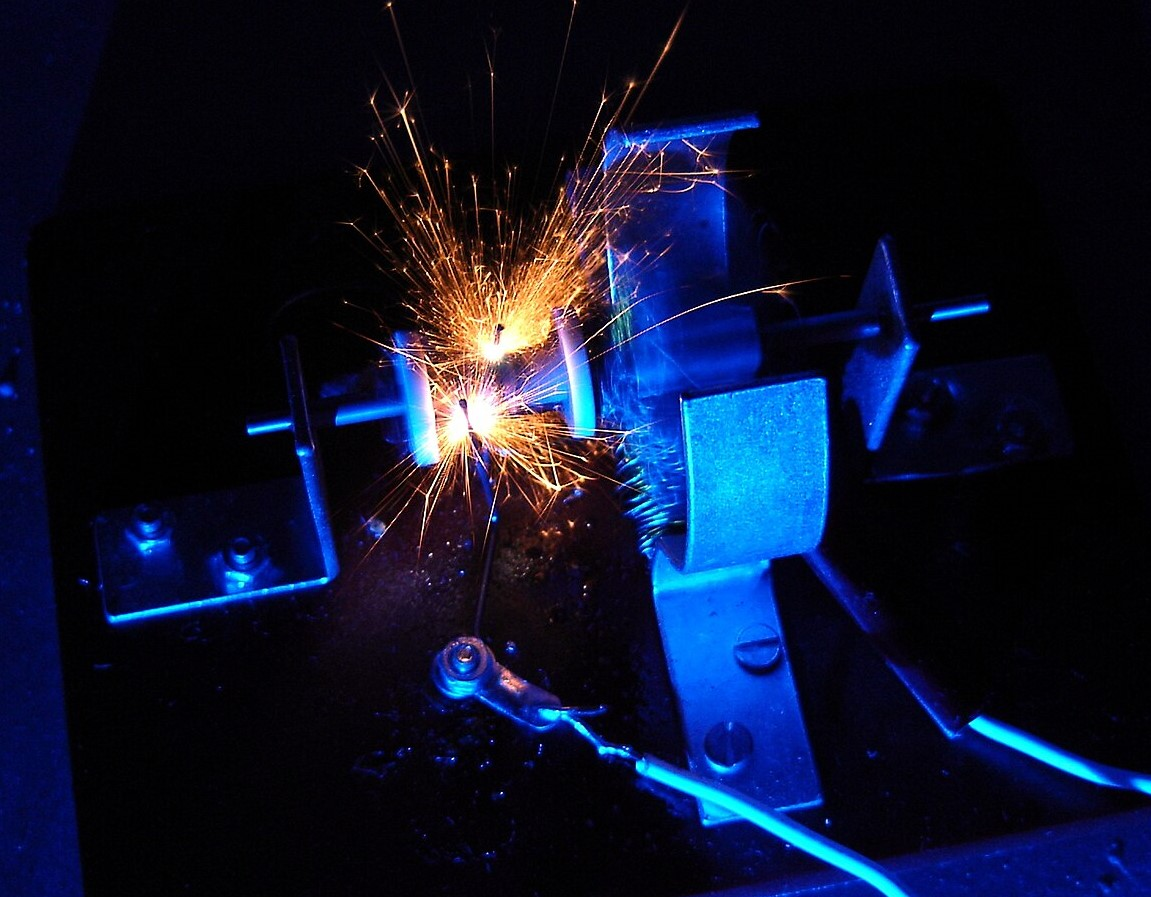
\includegraphics[width=0.95\textwidth]{fig/lec03/Commutator_sparking.jpg}
				\caption{Commutator sparking of a simple DC machine (source: \href{https://commons.wikimedia.org/wiki/File:Bürstenfeuer_eines_einfachen_Elektromotors.JPG}{Wikimedia Commons}, M. Frey, \href{https://creativecommons.org/licenses/by-sa/4.0/deed.den}{CC BY-SA 4.0})} 
				\label{fig:Commutator_sparking}
			\end{figure}
		\end{column}
		\begin{column}{0.6\textwidth}
			Assuming that the brush width $w_\mathrm{b}$ is much bigger than one commutator segment (which is usual practice), the commutation time $\Delta t_\mathrm{c}$ is given by
			\begin{equation}
				\Delta t_\mathrm{c} \approx \frac{w_\mathrm{b}}{v_\mathrm{c}}.
			\end{equation}\pause
			Here, $v_\mathrm{c}$ is the brush velocity
			\begin{equation}
				v_\mathrm{c} = \omega \frac{d_\mathrm{a}}{2}
			\end{equation}
			with the armature angular velocity $\omega$ and the armature diameter $d_\mathrm{a}$. \pause Due to the changing current in the coil, the so-called reactane voltage $u_\mathrm{r}$ is induced:
			\begin{equation}
				u_\mathrm{r} = L_\mathrm{c} \frac{\mathrm{d}i_\mathrm{c}}{\mathrm{d}t} \approx L_\mathrm{c} \frac{i_\mathrm{a}}{a \Delta t_\mathrm{c}} = L_\mathrm{c} i_\mathrm{a} \frac{\omega d_\mathrm{a}}{a w_\mathrm{b}2}.
				\label{eq:reactance_voltage_commutation}
			\end{equation}
		\end{column}
	\end{columns}
\end{frame}

%%%%%%%%%%%%%%%%%%%%%%%%%%%%%%%%%%%%%%%%%%%%%%%%%%%%%%%%%%%%%
%% Air gap field %%
%%%%%%%%%%%%%%%%%%%%%%%%%%%%%%%%%%%%%%%%%%%%%%%%%%%%%%%%%%%%%
\begin{frame}
	\frametitle{Air gap field}
	\begin{columns}
		\begin{column}{0.65\textwidth}
			\textbf{Assumption}: The air gap field distribution is homogenous and without any leakage (cf. \figref{fig:Ideal_air_gap_field}).\\ \onslide<2->{Consequently, we model the magnetic machine behavior with the simplified network shown in \figref{fig:Simplified_magnetic_network_DC_machine}.}% 
			\begin{figure}
				\centering
				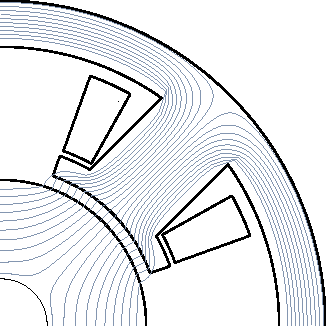
\includegraphics[width=0.4\textwidth]{fig/lec03/Ideal_air_gap_field.pdf}
				\caption{Idealized field lines (adapted from W.~Novender, \textit{Elektrische Maschinen}, Technische Hochschule Mittelhessen, 2023)}
				\label{fig:Ideal_air_gap_field}
			\end{figure}
		\end{column}
		\hfill
		\begin{column}{0.33\textwidth}
			\onslide<2->{\begin{figure}
				\centering
				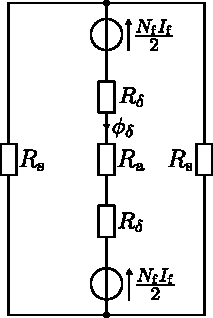
\includegraphics[height=0.65\textheight]{fig/lec03/Simplified_magnetic_network_DC_machine.pdf}
				\caption{Simplified magnetic network of a DC machine}
				\label{fig:Simplified_magnetic_network_DC_machine}
			\end{figure}}%
		\end{column}
	\end{columns}
\end{frame}

%%%%%%%%%%%%%%%%%%%%%%%%%%%%%%%%%%%%%%%%%%%%%%%%%%%%%%%%%%%%%
%% Air gap field (cont.) %%
%%%%%%%%%%%%%%%%%%%%%%%%%%%%%%%%%%%%%%%%%%%%%%%%%%%%%%%%%%%%%
\begin{frame}
	\frametitle{Air gap field (cont.)}
	\begin{columns}
		\begin{column}{0.65\textwidth}
			We introduce the following magnetic reluctances
			\begin{equation}
				\begin{alignedat}{2}
					R_\mathrm{s} &= \frac{l_\mathrm{s}}{\mu_{\mathrm{r, fe}} \mu_0  A_\mathrm{s}} \quad  &&(\mbox{stator reluctance}), \\ \quad R_\mathrm{a} &= \frac{l_\mathrm{a}}{\mu_{\mathrm{r, fe}}\mu_0  A_\mathrm{a}} \quad  &&(\mbox{armature reluctance}), \\
					R_\delta &= \frac{\delta}{\mu_0 A_\delta} \quad  &&(\mbox{air gap reluctance}).
				\end{alignedat}
			\end{equation}
			Above $l_i$ and $A_i$ are the respective lengths and cross-sectional areas of the field paths while $\delta$ is the air gap width. \onslide<2->{Furthermore, we have 
			$$ \mu_{\mathrm{r},\delta} = 1, \qquad \mu_{\mathrm{r, fe}} >> 1 .$$}%
		\end{column}
		\hfill
		\begin{column}{0.35\textwidth}
			\begin{figure}
				\centering
				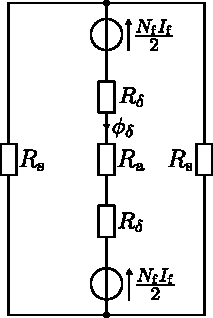
\includegraphics[height=0.65\textheight]{fig/lec03/Simplified_magnetic_network_DC_machine.pdf}
			\end{figure}
		\end{column}
	\end{columns}
\end{frame}

%%%%%%%%%%%%%%%%%%%%%%%%%%%%%%%%%%%%%%%%%%%%%%%%%%%%%%%%%%%%%
%% Air gap field (cont.) %%
%%%%%%%%%%%%%%%%%%%%%%%%%%%%%%%%%%%%%%%%%%%%%%%%%%%%%%%%%%%%%
\begin{frame}
	\frametitle{Air gap field (cont.)}
	\begin{columns}
		\begin{column}{0.65\textwidth}
			With $N_\mathrm{f}$ field winding turns and the field current $I_\mathrm{f}$, the air gap flux is given by:
			\begin{equation}
				\begin{split}
				\phi_\delta &= \frac{N_\mathrm{f} I_\mathrm{f}}{2 R_\delta + R_\mathrm{a} + \frac{1}{2}R_\mathrm{s}}\\
							& = \mu_0 N_\mathrm{f} I_\mathrm{f}\left(2\frac{\delta}{A_\delta} + \frac{l_\mathrm{a}}{\mu_{\mathrm{r, Fe}} A_\mathrm{a}} + \frac{1}{2}\frac{l_\mathrm{s}}{\mu_{\mathrm{r, Fe}} A_\mathrm{s}}\right)^{-1}. 
			\end{split}
			\label{eq:Air_gap_flux_DC_machine_simple}
			\end{equation}
			\onslide<2->{While the relative permeability of the iron paths is depending on the magnetic flux ($\mu_{\mathrm{r, Fe}} = \mu_{\mathrm{r, Fe}}(\phi)$) due to saturation (cf. \figref{fig:Permeability_of_ferromagnet}) rendering \eqref{eq:Air_gap_flux_DC_machine_simple} a nonlinear equation, we will assume that the air gap reluctance is dominating 
			\begin{equation}
				 R_\delta >> \left\{R_\mathrm{a}, R_\mathrm{s} \right\} .
				 \label{eq:DC_flux_reluctance_simpl}
			\end{equation}}%
		\end{column}
		\hfill
		\begin{column}{0.35\textwidth}
			\begin{figure}
				\centering
				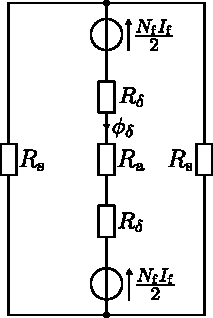
\includegraphics[height=0.65\textheight]{fig/lec03/Simplified_magnetic_network_DC_machine.pdf}
			\end{figure}
		\end{column}
	\end{columns}
\end{frame}

%%%%%%%%%%%%%%%%%%%%%%%%%%%%%%%%%%%%%%%%%%%%%%%%%%%%%%%%%%%%%
%% Air gap field (cont.) %%
%%%%%%%%%%%%%%%%%%%%%%%%%%%%%%%%%%%%%%%%%%%%%%%%%%%%%%%%%%%%%
\begin{frame}
	\frametitle{Air gap field (cont.)}
	Based on \eqref{eq:Air_gap_flux_DC_machine_simple} together with \eqref{eq:DC_flux_reluctance_simpl} we can simplify the effective air gap flux to
	\begin{equation}
		\phi_\delta = \frac{N_\mathrm{f} I_\mathrm{f}}{2 R_\delta} = \frac{N_\mathrm{F} I_\mathrm{f}}{2 \frac{\delta}{\mu_0 A_\delta}} = \frac{\mu_0 N_\mathrm{f} A_\delta}{2 \delta} I_\mathrm{f}.
		\label{eq:Air_gap_flux_DC_machine}
	\end{equation}\pause
	Here, $\delta$ is the air gap width and $A_\delta$ the effective cross-sectional area of the air gap which is
	\begin{equation}
		A_\delta = \alpha p \tau_\mathrm{p} l_z .
		\label{eq:Air_gap_area_DC_machine}
	\end{equation}\pause
	Above, the following assumptions and definitions are made:
	\begin{itemize}
		\item $l_z$ is the axial length of the machine. \pause
		\item The air gap width is very small such that the pole pitch $\tau_\mathrm{p}$ can be used as a good approximation for the air gap  circumference. \pause
		\item $\alpha$ is the pole coverage, that is, the ratio of the active pole surfaces to the pole pitch (cf. \figref{fig:Magnetic_field_normal_component_DC_machine} on next slide) representing the average field density in the air gap.
	\end{itemize}
\end{frame}

%%%%%%%%%%%%%%%%%%%%%%%%%%%%%%%%%%%%%%%%%%%%%%%%%%%%%%%%%%%%%
%% Air gap field (cont.) %%
%%%%%%%%%%%%%%%%%%%%%%%%%%%%%%%%%%%%%%%%%%%%%%%%%%%%%%%%%%%%%
\begin{frame}
	\frametitle{Air gap field (cont.)}
    \begin{figure}
        \centering
        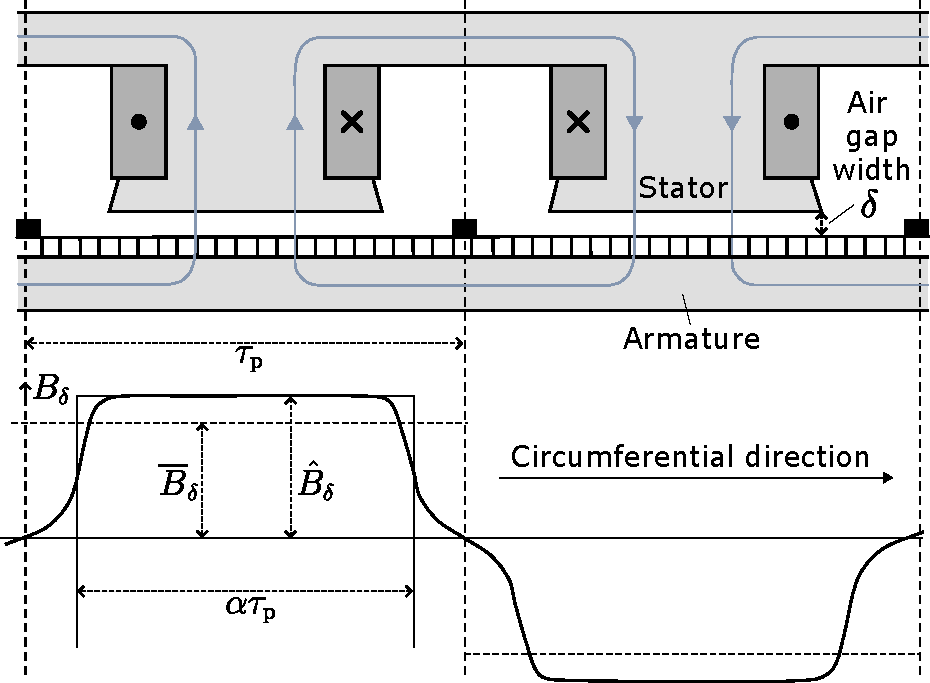
\includegraphics[height=0.67\textheight]{fig/lec03/Magnetic_field_normal_component_DC_machine.pdf}
        \caption{Principle magnetic field paths through stator and rotor as well as the (idealized) normal component of the magnetic field density $B_\delta$ in the air gap  (inspired from A. Binder, \textit{Elektrische Maschinen und Antriebe}, Vol. 2, Springer, 2017)}
		\label{fig:Magnetic_field_normal_component_DC_machine}
    \end{figure}
\end{frame}

%%%%%%%%%%%%%%%%%%%%%%%%%%%%%%%%%%%%%%%%%%%%%%%%%%%%%%%%%%%%%
%% Torque %%
%%%%%%%%%%%%%%%%%%%%%%%%%%%%%%%%%%%%%%%%%%%%%%%%%%%%%%%%%%%%%
\begin{frame}
	\frametitle{Torque}
	\begin{columns}
	\begin{column}{0.45\textwidth}
    From \eqref{eq:Air_gap_flux_DC_machine} we can calculate the air gap flux density $\hat{B}_\delta$ per pole pair as
	\begin{equation}
		\hat{B}_\delta = \frac{\phi_\delta}{A_\delta} = \frac{\mu_0 N_\mathrm{f}}{2 \delta p} I_\mathrm{f}.
		\label{eq:Air_gap_flux_density_DC_machine}
	\end{equation}\pause
	Assuming that the magnetic field only flows through each armature conductor in a perpendicular direction (cf. \figref{fig:DC_machine_cross_section_force_torque}), the absolute Lorentz force per armature conductor is resulting in
	\begin{equation}
		F_\mathrm{c} =  \hat{B}_\delta l_z I_\mathrm{c}= \frac{\mu_0 N_\mathrm{f} l_z}{4 \delta p a}I_\mathrm{f} I_\mathrm{a}.
		\label{eq:Lorentz_force_DC_machine_conductor}
	\end{equation}
\end{column}
\hfill
\begin{column}{0.55\textwidth}
	\begin{figure}
		\centering
		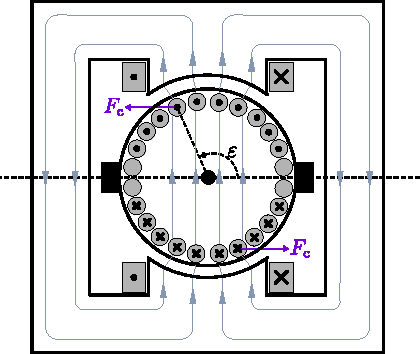
\includegraphics[width=0.725\textwidth]{fig/lec03/DC_machine_cross_section_force_torque.pdf}
		\caption{Simplified DC machine cross section with exemplary armature conductor force representation (adapted from J.~B\"ocker, \textit{Elektrische Antriebstechnik}, Paderborn University, 2020)}
		\label{fig:DC_machine_cross_section_force_torque}
	\end{figure}
\end{column}
\end{columns}
\end{frame}

%%%%%%%%%%%%%%%%%%%%%%%%%%%%%%%%%%%%%%%%%%%%%%%%%%%%%%%%%%%%%
%% Torque (cont.)%%
%%%%%%%%%%%%%%%%%%%%%%%%%%%%%%%%%%%%%%%%%%%%%%%%%%%%%%%%%%%%%
\begin{frame}
	\frametitle{Torque (cont.)}
	Assuming that the force direction acting on each armature conductor is perpendicular to the armature shaft, the torque per conductor for an armature diameter $d_\mathrm{a}$ is
	\begin{equation}
		T_\mathrm{c} = F_\mathrm{c} \frac{d_\mathrm{a}}{2} = \frac{\mu_0 N_\mathrm{f} l_z d_\mathrm{a}}{8 \delta p a} I_\mathrm{f} I_\mathrm{a}.
		\label{eq:Torque_DC_machine_conductor}
	\end{equation} \pause
	The resulting (average) machine torque $T$ for $N_\mathrm{a}$ armature conductor loops from which an $\alpha$  share is covered by the poles (cf. \figref{fig:Magnetic_field_normal_component_DC_machine}) is
	\begin{equation}
		\begin{split}
			\onslide<2->{T 	&= 2 \alpha N_\mathrm{a}  T_\mathrm{c} = \frac{\mu_0 \alpha N_\mathrm{f} N_\mathrm{a} l_z d_\mathrm{a}}{4 \delta p a} I_\mathrm{f} I_\mathrm{a} .} 
		\end{split}
	\end{equation}
	With $\tau_\mathrm{p} = \pi d_\mathrm{s}/(2 p) = \pi d_\mathrm{a}/(2 p)$ assuming a very small air gap width $\delta$ (cf. \figref{fig:DC_machine_cross_section_two_pole_pairs}) we can also rewrite the torque as
	\begin{equation}
		T = \frac{\mu_0 \alpha N_\mathrm{f} N_\mathrm{a} l_z \tau_\mathrm{p}}{2 \pi  \delta a} I_\mathrm{f} I_\mathrm{a}.
		\label{eq:Torque_DC_machine}
	\end{equation}\pause
\end{frame}


%%%%%%%%%%%%%%%%%%%%%%%%%%%%%%%%%%%%%%%%%%%%%%%%%%%%%%%%%%%%%
%% Effective field inductance and effective flux linkage %%
%%%%%%%%%%%%%%%%%%%%%%%%%%%%%%%%%%%%%%%%%%%%%%%%%%%%%%%%%%%%%
\begin{frame}
	\frametitle{Effective field inductance and effective flux linkage}
    To write \eqref{eq:Torque_DC_machine} more compact, we introduce the effective field inductance 
	\begin{equation}
		L_\mathrm{f}' =  \frac{\mu_0 \alpha N_\mathrm{f} N_\mathrm{a} l_z d_\mathrm{a}}{4 \delta p a } = \frac{\mu_0 \alpha N_\mathrm{f} N_\mathrm{a} l_z \tau_\mathrm{p}}{2 \pi  \delta a}.
		\label{eq:Effective_field_inductance}
	\end{equation} \pause
	Compared to the self-inductance of the field winding 
	\begin{equation}
		L_\mathrm{f} = \frac{N_\mathrm{f}^2}{2 R_\delta} = \frac{\mu  \alpha p \tau_\mathrm{p} l_z N_\mathrm{f}^2}{4 \delta},
	 \end{equation} \pause
	 we find
	 \begin{equation}
		 L_\mathrm{f}' = \underbrace{\frac{2p}{a \pi}\frac{N_\mathrm{a}}{N_\mathrm{f}}}_{c} L_\mathrm{f}  = c L_\mathrm{f} .
	\end{equation} \pause
	Finally, we define the effective field flux linkage $\psi_\mathrm{f}'$ to rewrite the torque expression
	\begin{equation}
		\psi_\mathrm{f}' = L_\mathrm{f}' I_\mathrm{f}, \hspace{1cm} T = c L_\mathrm{f} I_\mathrm{f} I_\mathrm{a} = L_\mathrm{f}' I_\mathrm{f} I_\mathrm{a}  = \psi_\mathrm{f}' I_\mathrm{a}.
		\label{eq:Effective_field_flux_linkage}
	\end{equation}
\end{frame}

%%%%%%%%%%%%%%%%%%%%%%%%%%%%%%%%%%%%%%%%%%%%%%%%%%%%%%%%%%%%%
%% Flux linkage of a single armature coil %%
%%%%%%%%%%%%%%%%%%%%%%%%%%%%%%%%%%%%%%%%%%%%%%%%%%%%%%%%%%%%%
\begin{frame}
	\frametitle{Flux linkage of a single armature coil}
	\begin{columns}
		\begin{column}{0.45\textwidth}
			From  \figref{fig:Magnetic_field_normal_component_DC_machine} we assume the air gap flux density normal component along $\varepsilon$ to be:
			\begin{equation}
				B(\varepsilon) = \begin{cases}
					\overline{B}_\delta, &  0 \leq \varepsilon < \pi,\\
					-\overline{B}_\delta, &  \pi \leq \varepsilon < 2\pi.
				\end{cases}
				\label{eq:Air_gap_flux_density_DC_machine_circumference}
			\end{equation}
			The flux linkage of a single armature coil starting at position $\varepsilon$ is then
			\begin{equation}
				\begin{split}
				\phi_\mathrm{c}(\varepsilon) &= \iint_{S} \bm{B} \cdot \mathrm{d}\bm{S}
											 = l_\mathrm{z}d_\mathrm{a}\int_{\varepsilon}^{\varepsilon+\pi}B(\varepsilon) \mathrm{d}\varepsilon \\
											 & = l_\mathrm{z}d_\mathrm{a}\overline{B}_\delta\begin{cases}
												(\pi/2 - \varepsilon), &  0 \leq \varepsilon < \pi,\\
												(\varepsilon - 3\pi/2), &  \pi \leq \varepsilon < 2\pi.
											\end{cases}.
				\end{split}
				\label{eq:Flux_linkage_single_coil}
			\end{equation}
		\end{column}
	\hfill
	\begin{column}{0.55\textwidth}
		\begin{figure}
			\centering
			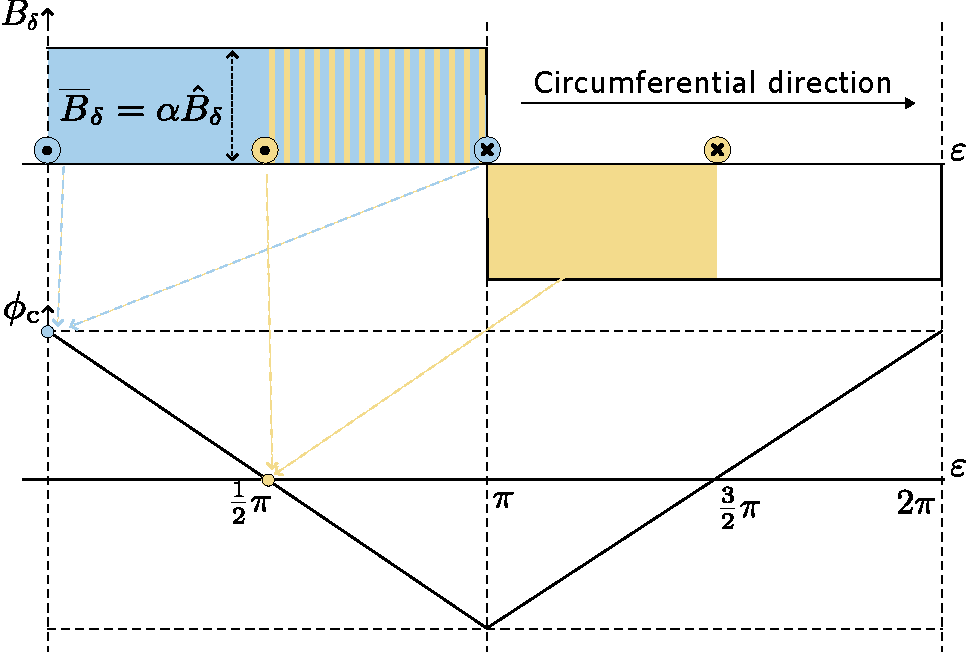
\includegraphics[height=0.6\textheight]{fig/lec03/Flux_density_and_linkage.pdf}
			\caption{Flux linkage $\psi_\mathrm{c}$ of a single armature coil based on the simplified, rectangular air gap flux density $B_\delta(\varepsilon)$  from \figref{fig:Magnetic_field_normal_component_DC_machine} -- light blue and yellow areas represent two exemplary armature coil positions.}
			\label{fig:Flux_density_and_linkage}
		\end{figure}
	\end{column}
	\end{columns}
\end{frame}

%%%%%%%%%%%%%%%%%%%%%%%%%%%%%%%%%%%%%%%%%%%%%%%%%%%%%%%%%%%%%
%% Induced voltage %%
%%%%%%%%%%%%%%%%%%%%%%%%%%%%%%%%%%%%%%%%%%%%%%%%%%%%%%%%%%%%%
\begin{frame}
	\frametitle{Induced voltage}
	Assuming that the armature is rotating with the (constant) speed $n$ (or angular velocity $\omega = 2 \pi n=\dot{\varepsilon}$), the induced voltage per armature conductor loop is
	\begin{equation}
			u_\mathrm{i,c} = - \frac{\mathrm{d}}{\mathrm{d}t} \phi_\mathrm{c} = - \frac{\mathrm{d}}{\mathrm{d}\varepsilon} \phi_\mathrm{c} \frac{\mathrm{d}}{\mathrm{d}t}\varepsilon = - \omega l_\mathrm{z}d_\mathrm{a}\overline{B}_\delta \begin{cases}
				-\omega, &  0 \leq \varepsilon < \pi,\\
				\omega, &  \pi \leq \varepsilon < 2\pi.
			\end{cases}
		\label{eq:Induced_voltage_per_conductor}
	\end{equation}
	To calculate the total induced voltage $u_\mathrm{i}$, we consider
	\begin{itemize}
	   \item the rectification of the induced voltage by the commutator, \pause 		
	   \item $N_\mathrm{a}$ total armature conductor loops, \pause
	   \item $2 a$ parallel armature conductors per pole pair (depends on winding scheme, cf. \eqref{eq:Parallel_conductors}), \pause
	\end{itemize}
	resulting in: \pause
	\begin{equation}
			u_\mathrm{i} = \frac{N_\mathrm{a}}{2 a} |u_\mathrm{i,c}| = \frac{N_\mathrm{a}}{2 a}\omega l_\mathrm{z}d_\mathrm{a}\overline{B}_\delta = \omega I_\mathrm{f}\frac{\mu_0 \alpha N_\mathrm{f} N_\mathrm{a} l_\mathrm{z} d_\mathrm{a}}{4 \delta p a} =  \omega I_\mathrm{f} \frac{\mu_0 \alpha N_\mathrm{f} N_\mathrm{a} l_z \tau_\mathrm{p}}{2 \pi  \delta a} =\omega I_\mathrm{f} L_\mathrm{f}' = \omega  \psi_\mathrm{f}'.
	\end{equation}
\end{frame}


%%%%%%%%%%%%%%%%%%%%%%%%%%%%%%%%%%%%%%%%%%%%%%%%%%%%%%%%%%%%%
%% Equivalent circuit diagram and summary of important equations %%
%%%%%%%%%%%%%%%%%%%%%%%%%%%%%%%%%%%%%%%%%%%%%%%%%%%%%%%%%%%%%
\begin{frame}
	\frametitle{Equivalent circuit diagram and summary of important equations}
	\begin{columns}
		\begin{column}{0.55\textwidth}
	Field and armature voltage equations:
	\begin{equation}
		\begin{aligned}
			u_\mathrm{f} &= R_\mathrm{f} i_\mathrm{f} + L_\mathrm{f} \frac{\mathrm{d}i_\mathrm{f}}{\mathrm{d}t} \\
			u_\mathrm{a} &= R_\mathrm{a} i_\mathrm{a} + L_\mathrm{a} \frac{\mathrm{d}i_\mathrm{a}}{\mathrm{d}t} + u_\mathrm{i} 
		\end{aligned}
		 \label{eq:DC_machine_ODE_currents}
	\end{equation} \pause
	Induced voltage:
	\begin{equation*}
			u_\mathrm{i} = \omega \psi_\mathrm{f}' = \omega i_\mathrm{f} L_\mathrm{f}' 
	\end{equation*} \pause
	Torque:
	\begin{equation*}
		T =  L_\mathrm{f}' i_\mathrm{f} i_\mathrm{a}  = \psi_\mathrm{f}' i_\mathrm{a}
	\end{equation*} \pause
	\textbf{Note}: we represent the machine currents with small letters to indicate that they are time-dependent (e.g., if the external voltage supplied is varying).
\end{column} \pause
\hfill
\begin{column}{0.45\textwidth}
	\begin{figure}
		\centering
		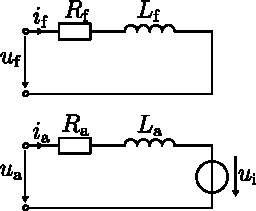
\includegraphics[width=0.8\textwidth]{fig/lec03/ECD_DC_machine.pdf}
		\caption{Equivalent circuit diagram of the DC machine}
		\label{fig:ECD_DC_machine}
	\end{figure}
\end{column}
\end{columns}
\end{frame}

%%%%%%%%%%%%%%%%%%%%%%%%%%%%%%%%%%%%%%%%%%%%%%%%%%%%%%%%%%%%%
%% Power balance and efficiency %%
%%%%%%%%%%%%%%%%%%%%%%%%%%%%%%%%%%%%%%%%%%%%%%%%%%%%%%%%%%%%%
\begin{frame}
	\frametitle{Power balance and efficiency}
		Based on \eqref{fig:ECD_DC_machine} (note the load convention), the electrical power of the DC machine is:
		\begin{equation}
			P_\mathrm{el} = u_\mathrm{a} i_\mathrm{a} + u_\mathrm{f} i_\mathrm{f}.
		\end{equation} \pause
		This power is separated into the mechanical power $P_\mathrm{me}$, the dissipated power losses $P_\mathrm{l}$, and the change of the stored magnetic energy $\frac{\mathrm{d}}{\mathrm{d}t}E_\mathrm{mag}$:
		\begin{equation}
			P_\mathrm{el} = P_\mathrm{me} + P_\mathrm{l} + \frac{\mathrm{d}}{\mathrm{d}t}E_\mathrm{mag}.
		\end{equation} \pause
		The power losses are (assuming dominant ohmic losses):
		\begin{equation}
			P_\mathrm{l} = R_\mathrm{f} i_\mathrm{f}^2 + R_\mathrm{a} i_\mathrm{a}^2.
		\end{equation} \pause
		The mechanical power is:
		\begin{equation}
			P_\mathrm{me} = T \omega = \psi_\mathrm{f}' i_\mathrm{a} \omega.
		\end{equation} \pause
		The magnetically stored energy is
		\begin{equation}
			E_\mathrm{mag} = \frac{1}{2} L_\mathrm{f} i_\mathrm{f}^2 + \frac{1}{2} L_\mathrm{a} i_\mathrm{a}^2.
		\end{equation}
\end{frame}

%%%%%%%%%%%%%%%%%%%%%%%%%%%%%%%%%%%%%%%%%%%%%%%%%%%%%%%%%%%%%
%% Power balance and efficiency %%
%%%%%%%%%%%%%%%%%%%%%%%%%%%%%%%%%%%%%%%%%%%%%%%%%%%%%%%%%%%%%
\begin{frame}
	\frametitle{Power balance and efficiency (cont.)}
		In steady state, the DC machine efficiency $\eta$ is defined as
		\begin{equation}
			\begin{split}
				\eta_{\mathrm{mot}} &= \frac{P_\mathrm{me}}{P_\mathrm{el}} = \frac{T \omega}{u_\mathrm{a} i_\mathrm{a} + u_\mathrm{f} i_\mathrm{f}} = \frac{L_\mathrm{f}' i_\mathrm{f}i_\mathrm{a}\omega}{R_\mathrm{a}i_\mathrm{a}^2 + \omega L_\mathrm{f}' i_\mathrm{f} i_\mathrm{a} +R_\mathrm{f}i_\mathrm{f}^2},\\[1em]
				\onslide<2->{\eta_{\mathrm{gen}} &= \frac{P_\mathrm{el}}{P_\mathrm{me}} = \frac{u_\mathrm{a} i_\mathrm{a} + u_\mathrm{f} i_\mathrm{f}}{T \omega} = \frac{R_\mathrm{a}i_\mathrm{a}^2 + \omega L_\mathrm{f}' i_\mathrm{f} i_\mathrm{a} +R_\mathrm{f}i_\mathrm{f}^2}{L_\mathrm{f}' i_\mathrm{f}i_\mathrm{a}\omega}.}
			\end{split}
		\end{equation}
		\onslide<3->{
		It can be noted that
		\begin{itemize}
			\item The machine parameters $R_\mathrm{a}$, $R_\mathrm{f}$, and $L_\mathrm{f}'$ are influencing the efficiency.}\onslide<4->{
			\item The efficiency is a function of the load torque $T$ and the speed $\omega$, that is, depending on the operating point.}\onslide<5->{
			\item If $i_\mathrm{f}$ and $i_\mathrm{a}$ are independently controllable, the efficiency can be optimized as a certain torque can be produced with infinitely many combinations of $i_\mathrm{f}$ and $i_\mathrm{a}$.}
		\end{itemize}
\end{frame}

%%%%%%%%%%%%%%%%%%%%%%%%%%%%%%%%%%%%%%%%%%%%%%%%%%%%%%%%%%%%%
%% Intermediate remarks on the DC machine model %%
%%%%%%%%%%%%%%%%%%%%%%%%%%%%%%%%%%%%%%%%%%%%%%%%%%%%%%%%%%%%%
\begin{frame}
	\frametitle{Intermediate remarks on the DC machine model} 
	During the derivation of the DC machine model, we made several assumptions:
	\begin{itemize}
		\item The air gap magnetic field is homogenous and without any leakage. \pause
		\item The air gap reluctance is dominating the magnetic circuit (neglecting the iron path reluctances including potential magnetic saturation).\pause
		\item The magnetic field lines follow distinct paths through the armature winding. \pause
		\item There is no mutual inductance between the stator and rotor (ideal orthogonal windings). \pause
		\item The magnetic field in the air gap and in the armature is governed by the field winding current only (that is, we have neglected the armature current impact on the field). \pause
	\end{itemize}
	\begin{varblock}{Model accuracy}
		We represent the DC machine by a time-invariant, lumped-parameter model which is based on several substantial simplifications. While this model is likely sufficient for many applications, systematic deviations between the observed behavior of real machines and the model predictions are to be expected.
	\end{varblock}
\end{frame}

%%%%%%%%%%%%%%%%%%%%%%%%%%%%%%%%%%%%%%%%%%%%%%%%%%%%%%%%%%%%%
%% Armature reaction %%
%%%%%%%%%%%%%%%%%%%%%%%%%%%%%%%%%%%%%%%%%%%%%%%%%%%%%%%%%%%%%
\begin{frame}
	\frametitle{Armature reaction}
	\begin{itemize}
		\item So far, we have neglected the impact of the armature current on the magnetic field.
		\item If $i_\mathrm{a}\neq 0$, the magnetic field lines in the air gap are distorted leading to a so-called armature reaction (cf. \figref{fig:Armature_reaction}).
	\end{itemize}
    \begin{figure}
        \centering
        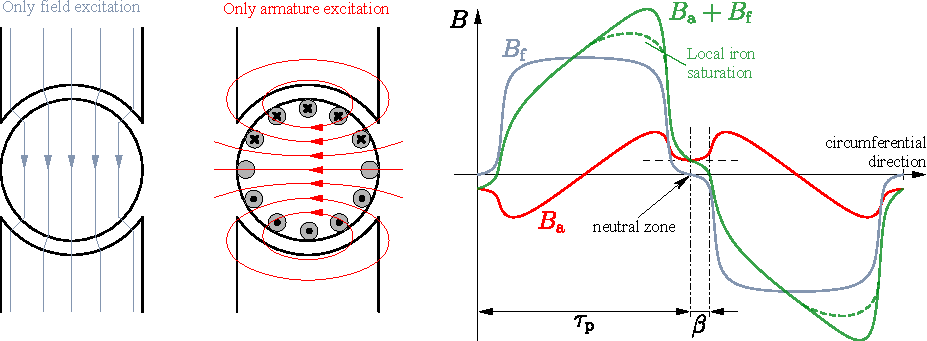
\includegraphics[width=0.75\textwidth]{fig/lec03/Armature_reaction.pdf}
        \caption{Superpostion of the field and armature magnetic excitation and the resulting air gap field normal components (adapted from W.~Novender, \textit{Elektrische Maschinen}, Technische Hochschule Mittelhessen, 2023)} 
		\label{fig:Armature_reaction}
    \end{figure}
\end{frame}

%%%%%%%%%%%%%%%%%%%%%%%%%%%%%%%%%%%%%%%%%%%%%%%%%%%%%%%%%%%%%
%% Armature reaction (cont.) %%
%%%%%%%%%%%%%%%%%%%%%%%%%%%%%%%%%%%%%%%%%%%%%%%%%%%%%%%%%%%%%
\begin{frame}
	\frametitle{Armature reaction (cont.)}
	\begin{columns}
		\begin{column}{0.55\textwidth}
	Issues related to the armature reaction:
	\begin{itemize}
		\item The neutral zone (field-free commutation area) is shifted by $\beta$ degrees in the circumferential direction, that is, exacerbate the commutation process (increased risk of sparking).
		\item<2-> High local field densities can lead to magnetic saturation which will increase the iron path reluctance and consequently decrease the machine's torque capability. Also, the iron losses will increase. 
		\item<3-> The imbalanced magnetic field leads to an imbalanced Lorentz force distribution on the armature conductors which can cause mechanical distortions. 
	\end{itemize}
\end{column}
\hfill
\begin{column}{0.45\textwidth}
	\begin{figure}
		\centering
		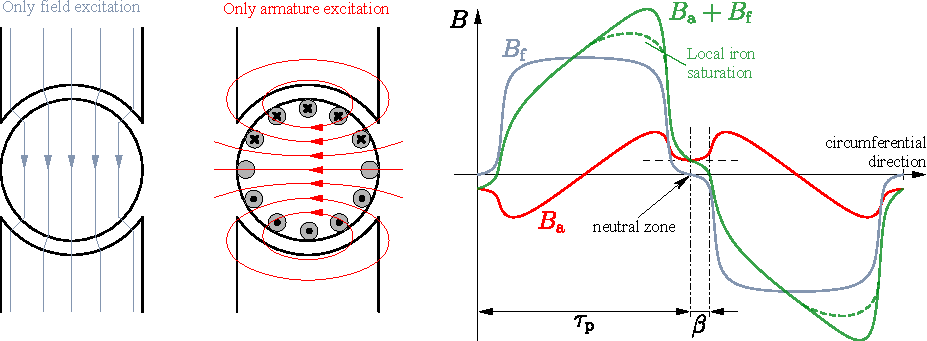
\includegraphics[trim={7.2cm 0 0 0}, clip, width=0.95\textwidth]{fig/lec03/Armature_reaction.pdf}
	\end{figure}
\end{column}
\end{columns}
\end{frame}

%%%%%%%%%%%%%%%%%%%%%%%%%%%%%%%%%%%%%%%%%%%%%%%%%%%%%%%%%%%%%
%% Counter measures: compensation winding and interpoles %%
%%%%%%%%%%%%%%%%%%%%%%%%%%%%%%%%%%%%%%%%%%%%%%%%%%%%%%%%%%%%%
\begin{frame}
	\frametitle{Counter measures: compensation winding and interpoles}
    \begin{figure}
        \centering
        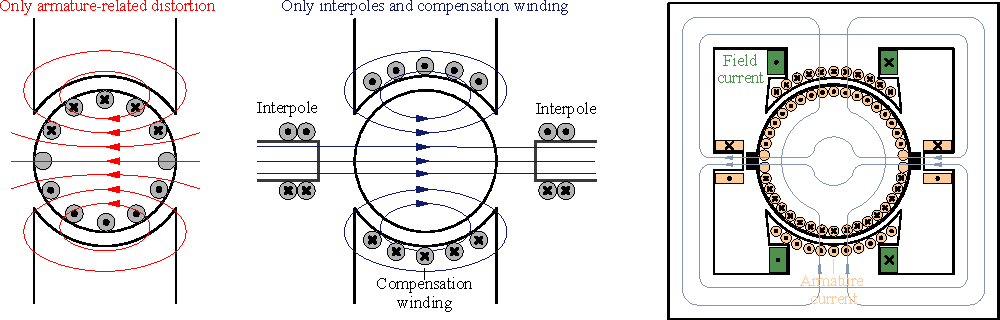
\includegraphics[width=0.9\textwidth]{fig/lec03/Compensation_winding_interpoles.pdf}
        \caption{Armature reaction counter measures utilizing compensation winding and interpoles: both are excited by the armature current with an opposite orientation to account for the load-dependent impact of the armature reaction (adapted from W.~Novender, \textit{Elektrische Maschinen}, Technische Hochschule Mittelhessen, 2023 and J.~B\"ocker, \textit{Elektrische Antriebstechnik}, Paderborn University, 2020)} 
		\label{fig:Compensation_winding_interpoles}
    \end{figure}
\end{frame}

%%%%%%%%%%%%%%%%%%%%%%%%%%%%%%%%%%%%%%%%%%%%%%%%%%%%%%%%%%%%%
%% Counter measures: compensation winding and interpoles %%
%%%%%%%%%%%%%%%%%%%%%%%%%%%%%%%%%%%%%%%%%%%%%%%%%%%%%%%%%%%%%
\begin{frame}
	\frametitle{Counter measures: compensation winding and interpoles (cont.)}
    \begin{figure}
        \centering
        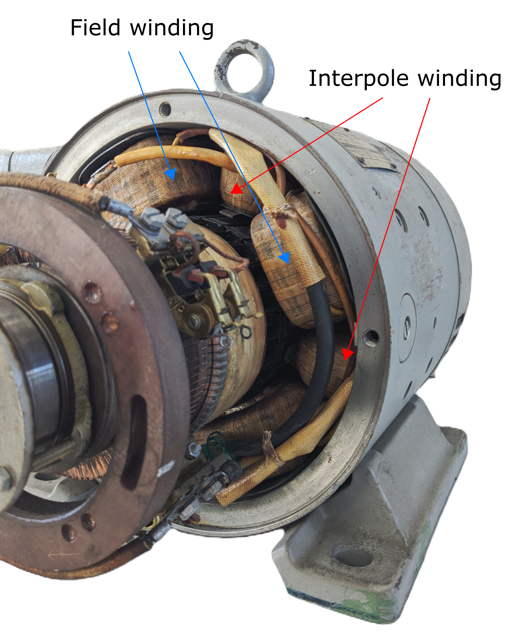
\includegraphics[height=0.70\textheight]{fig/lec03/Interpole_winding_example.png}
        \caption{Example of a DC machine with interpole winding (one may identify that the interpole winding is connected to the brushes and, therefore, excited by the armature current)}
		\label{fig:Interpole_winding_example}
    \end{figure}
\end{frame}

%%%%%%%%%%%%%%%%%%%%%%%%%%%%%%%%%%%%%%%%%%%%%%%%%%%%%%%%%%%%%
%% Counter measures: compensation winding and interpoles %%
%%%%%%%%%%%%%%%%%%%%%%%%%%%%%%%%%%%%%%%%%%%%%%%%%%%%%%%%%%%%%
\begin{frame}
	\frametitle{Counter measures: compensation winding and interpoles (cont.)}
   \textbf{Compensation winding design:}
   In order to compensate for the armature reaction within the air gap, the compensation winding MMF $\theta_\mathrm{cw}$ must meet the armature MMF $\theta_\mathrm{a}$:
   \begin{equation}
	   |\theta_\mathrm{cw}| = \frac{z_\mathrm{cw}}{2 a_\mathrm{cw} p }  I_\mathrm{a} \stackrel{!}{=} \alpha \frac{z_\mathrm{a}}{2 a_\mathrm{a} p } I_\mathrm{a} =|\theta_\mathrm{a}|.
	   \label{eq:MMF_compensation_winding}
	\end{equation}
	Above, the following parameters are used:
	\begin{itemize}
		\item $a_\mathrm{cw} / a_\mathrm{a}$: number of parallel conductors of the compensation and armature windings,
		\item $z_\mathrm{cw} / z_\mathrm{a}$: number of conductors of the compensation  and armature windings.
	\end{itemize} \pause
	In \eqref{eq:MMF_compensation_winding} $\alpha$ is only related to $\theta_\mathrm{a}$ as we assume the armature area to be bigger (or at least the same size) as the field pole (cf. \figref{fig:Compensation_winding_interpoles}). \pause From \eqref{eq:MMF_compensation_winding} we can calculate the required compensation winding conductors
	\begin{equation}
		z_\mathrm{cw} = \alpha z_\mathrm{a} \frac{a_\mathrm{cw}}{a_\mathrm{a}} =  2p Q_\mathrm{cw} N_\mathrm{cw}
	\end{equation}
	which can be met by choosing $Q_\mathrm{cw}$ slots and $N_\mathrm{cw}$ turns per pole.
\end{frame}

%%%%%%%%%%%%%%%%%%%%%%%%%%%%%%%%%%%%%%%%%%%%%%%%%%%%%%%%%%%%%
%% Counter measures: compensation winding and interpoles %%
%%%%%%%%%%%%%%%%%%%%%%%%%%%%%%%%%%%%%%%%%%%%%%%%%%%%%%%%%%%%%
\begin{frame}
	\frametitle{Counter measures: compensation winding and interpoles (cont.)}
   \textbf{Interpole winding design:}
   As discussed in \eqref{eq:reactance_voltage_commutation}, the reactane voltage $u_\mathrm{r} \approx  L_\mathrm{c} i_\mathrm{a} \omega d_\mathrm{a} / (a w_\mathrm{b}2)$ is self-induced within the short-circuited coil during commutation. To counteract this, the interpole winding is designed such that the neutral zone is (over-)compensated leading to an induced voltage $u_\mathrm{ip}$ which is opposite to $u_\mathrm{r}$:
   \begin{equation}
	   |u_\mathrm{ip}| \stackrel{!}{=} |u_\mathrm{r}|.
	   \label{eq:Interpole_voltage_condition}
	\end{equation} \pause
	Assuming a rotational angular velocity $\omega$ and some (homogenous) $B_\mathrm{ip}\neq 0$ flux density in the interpole area, the induced voltage $u_\mathrm{ip}$ is
	\begin{equation}
		u_\mathrm{ip} =  N_\mathrm{c} \omega d_\mathrm{a} l_\mathrm{z} B_\mathrm{ip}.
		\label{eq:Induced_voltage_interpole}
	 \end{equation} 
	 Here, $N_\mathrm{c}$ is the number of armature conductor turns per coil assuming that exatly one coil is placed in the interpole area. 
\end{frame}

%%%%%%%%%%%%%%%%%%%%%%%%%%%%%%%%%%%%%%%%%%%%%%%%%%%%%%%%%%%%%
%% Counter measures: compensation winding and interpoles %%
%%%%%%%%%%%%%%%%%%%%%%%%%%%%%%%%%%%%%%%%%%%%%%%%%%%%%%%%%%%%%
\begin{frame}
	\frametitle{Counter measures: compensation winding and interpoles (cont.)}
	\begin{columns}
		\begin{column}{0.55\textwidth}
			From \eqref{eq:Interpole_voltage_condition} and \eqref{eq:Induced_voltage_interpole} we can calculate the required interpole flux density $B_\mathrm{ip}$:
			\begin{equation}
				B_\mathrm{ip} = \frac{u_\mathrm{r}}{N_\mathrm{c} \omega d_\mathrm{a} l_\mathrm{z}} = \frac{L_\mathrm{c}i_\mathrm{a}}{2 N_\mathrm{c} l_\mathrm{z} a w_\mathrm{b}}.
				\label{eq:Interpole_flux_density}
			\end{equation}
			\onslide<2->{Applying the compensation winding design approach \eqref{eq:MMF_compensation_winding} results in:
			\begin{equation}
					\oint_{\partial S} \bm{H} \cdot \mathrm{d}\bm{s} = \theta_\mathrm{ip} +\theta_\mathrm{cw}-\theta_\mathrm{a} = \theta_\mathrm{ip}-\theta_\mathrm{a}(1-\alpha). 
			\end{equation} }\onslide<3->{The MMFs per pole are:
			\begin{equation}
				\theta_\mathrm{ip} = N_\mathrm{ip} i_\mathrm{a} , \qquad \theta_\mathrm{a}= N_\mathrm{a} i_\mathrm{a}.
			\end{equation}}
\end{column}
\hfill
\begin{column}{0.45\textwidth}
	\vspace{-0.2cm}
	\begin{figure}
		\centering
		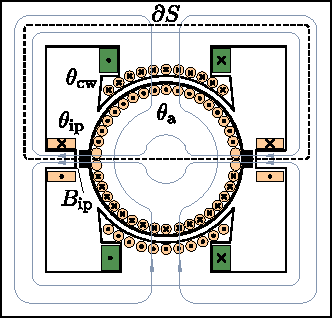
\includegraphics[width=0.8\textwidth]{fig/lec03/Interpole_integration_contour.pdf}
		\caption{Integration contour $\partial S$ and related MMF components for the interpole winding design (adapted from J.~B\"ocker, \textit{Elektrische Antriebstechnik}, Paderborn University, 2020)}
		\label{fig:Interpole_integration_contour}
	\end{figure}
\end{column}
\end{columns}
\end{frame}

%%%%%%%%%%%%%%%%%%%%%%%%%%%%%%%%%%%%%%%%%%%%%%%%%%%%%%%%%%%%%
%% Counter measures: compensation winding and interpoles %%
%%%%%%%%%%%%%%%%%%%%%%%%%%%%%%%%%%%%%%%%%%%%%%%%%%%%%%%%%%%%%
\begin{frame}
	\frametitle{Counter measures: compensation winding and interpoles (cont.)}
	\begin{columns}
		\begin{column}{0.55\textwidth}
		Assuming that the air gap reluctance is dominating the magnetic circuit, we  receive
			\begin{equation}
				\oint_{\partial S} \bm{H} \cdot \mathrm{d}\bm{s} = 2 \delta H_\mathrm{ip} = N_\mathrm{ip} i_\mathrm{a} - N_\mathrm{a} i_\mathrm{a}(1-\alpha).
			\end{equation}
		\onslide<2->{The flux density in the interpole area is then
		\begin{equation}
			B_\mathrm{ip} = \mu_0 \frac{N_\mathrm{ip}  - N_\mathrm{a} (1-\alpha)}{2 \delta} i_\mathrm{a}.
		\end{equation}}
		\onslide<3->{The comparison with \eqref{eq:Interpole_flux_density} reveals:
		\begin{equation}
			\begin{split}
				&\mu_0 \frac{N_\mathrm{ip}  - N_\mathrm{a} (1-\alpha)}{2 \delta} i_\mathrm{a} \stackrel{!}{=} \frac{L_\mathrm{c}}{2 N_\mathrm{c} l_\mathrm{z} a w_\mathrm{b}} i_\mathrm{a}\\}
				\onslide<4->{\Leftrightarrow \quad &N_\mathrm{ip}  = N_\mathrm{a} (1-\alpha) + \frac{ L_\mathrm{c}\delta}{\mu_0 N_\mathrm{c} l_\mathrm{z} a w_\mathrm{b}}.}
			\end{split}
		\end{equation}
\end{column}
\hfill
\begin{column}{0.45\textwidth}
	\vspace{-0.2cm}
	\onslide<1->{
	\begin{figure}
		\centering
		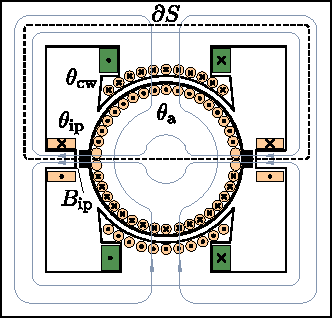
\includegraphics[width=0.8\textwidth]{fig/lec03/Interpole_integration_contour.pdf}
	\end{figure}}
\end{column}
\end{columns}
\end{frame}



%%%%%%%%%%%%%%%%%%%%%%%%%%%%%%%%%%%%%%%%%%%%%%%%%%%%%%%%%%%%%
%% Connection types of DC machines %%
%%%%%%%%%%%%%%%%%%%%%%%%%%%%%%%%%%%%%%%%%%%%%%%%%%%%%%%%%%%%%
\begin{frame}
	\frametitle{Connection types of DC machines}
	\vspace{-0.1cm}
	\begin{figure}
		\ContinuedFloat
		\centering
		\begin{subfigure}[b]{0.49\textwidth}
			\centering
			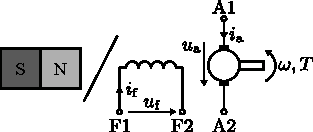
\includegraphics[scale=1.2]{fig/lec03/Separately_excited_DC_machine.pdf}
			\caption{Separately excited (or perm. magnet) DC machine} 
		\end{subfigure}
		\hfill
		\begin{subfigure}[b]{0.49\textwidth}
			\centering
			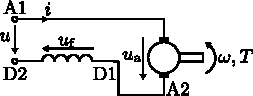
\includegraphics[scale=1.2]{fig/lec03/Series_DC_machine.pdf}
			\caption{Series DC machine} 
		\end{subfigure}
		\\
		\begin{subfigure}[b]{0.49\textwidth}
			\centering
			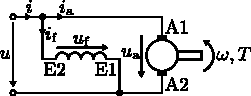
\includegraphics[scale=1.2]{fig/lec03/Shunt_DC_machine.pdf}
			\caption{Shunt DC machine} 
		\end{subfigure}
		\hfill
		\begin{subfigure}[b]{0.49\textwidth}
			\centering
			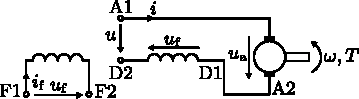
\includegraphics[scale=1.2]{fig/lec03/Compound_DC_machine.pdf}
			\caption{Compound DC machine} 
		\end{subfigure}
		\vspace{-0.1cm}
		\caption{Connection types of DC machines incl. terminal block designations (note: the not shown interpole winding has the terminal block designation $\mbox{B}1$-$\mbox{B}2$ and the compensation winding $\mbox{C}1$-$\mbox{C}2$)} 
        \label{fig:connection_types_DC_machines}
	\end{figure}
\end{frame}

%%%%%%%%%%%%%%%%%%%%%%%%%%%%%%%%%%%%%%%%%%%%%%%%%%%%%%%%%%%%%
%% Steady-state behavior: separately excited DC machine %%
%%%%%%%%%%%%%%%%%%%%%%%%%%%%%%%%%%%%%%%%%%%%%%%%%%%%%%%%%%%%%
\begin{frame}
	\frametitle{Steady-state behavior: separately excited DC machine}
			Assuming a fixed excitation $\psi_\mathrm{f}'$ (e.g., by a permanent magnet or constant field current), the separately excited DC machine's voltage demand for a certain speed is:
			\begin{equation}
				U_\mathrm{a} = R_\mathrm{a} I_\mathrm{a} + \omega \psi_\mathrm{f}'.
			\end{equation} \pause
			On the other hand, the speed-torque characteristic for a fixed armature voltage supply $U_\mathrm{a}$ is
			\begin{equation}
				T = \left(U_\mathrm{a} -\omega \psi_\mathrm{f}'\right)\frac{\psi_\mathrm{f}'}{R_\mathrm{a}} = U_\mathrm{a}\frac{\psi_\mathrm{f}'}{R_\mathrm{a}} - \omega \frac{\psi_\mathrm{f}'^2}{R_\mathrm{a}}.
			\end{equation}\pause
		\begin{figure}
		\begin{columns}
			\begin{column}{0.7\textwidth}
				\centering
				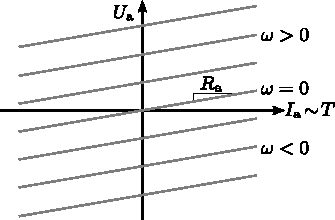
\includegraphics[height=0.4\textheight]{fig/lec03/Sep_DC_machine_voltage_current.pdf}\hspace{0.5cm}
				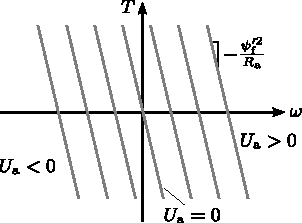
\includegraphics[height=0.4\textheight]{fig/lec03/Sep_DC_machine_torque_speed.pdf}
			\end{column}
			\begin{column}{0.3\textwidth}
				\caption{\raggedright Steady-state characteristics curves (adapted from J.~B\"ocker, \textit{Elektrische Antriebstechnik}, Paderborn University, 2020)}
				\label{fig:char_curves_steady_state_sep_DC_machine}
			\end{column}
		\end{columns}
		\end{figure}
\end{frame}

%%%%%%%%%%%%%%%%%%%%%%%%%%%%%%%%%%%%%%%%%%%%%%%%%%%%%%%%%%%%%
%% Steady-state behavior: separately excited DC machine (cont.) %%
%%%%%%%%%%%%%%%%%%%%%%%%%%%%%%%%%%%%%%%%%%%%%%%%%%%%%%%%%%%%%
\begin{frame}
	\frametitle{Steady-state behavior: separately excited DC machine (cont.)}
	\begin{columns}
		\begin{column}{0.55\textwidth}
		For $U_\mathrm{a}=\mbox{const.}>0$, the starting torque (i.e., the torque at zero speed) and the corresponding armature current are:
		\begin{equation}
			\begin{split}
				T(\omega=0) &= T_0 = U_\mathrm{a}\frac{\psi_\mathrm{f}'}{R_\mathrm{a}}, \\ I_\mathrm{a}(\omega=0) &= I_{\mathrm{a}0}=  \frac{U_\mathrm{a}}{R_\mathrm{a}}.
			\end{split}
		\end{equation} \pause
		On the other hand for $T=0$, the no-load speed $\omega_0$ is:
		\begin{equation}
			\omega_0 = \frac{U_\mathrm{a}}{\psi_\mathrm{f}'}.
		\end{equation} \pause
\end{column}
\hfill
\begin{column}{0.45\textwidth}
	\vspace{-0.2cm}
	\begin{figure}
		\centering
		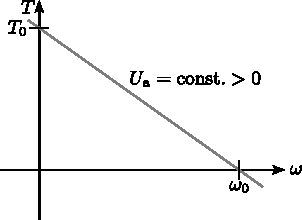
\includegraphics{fig/lec03/Sep_DC_machine_starting_torque.pdf}
		\caption{Starting torque and no-load speed of a separately excited DC machine (adapted from J.~B\"ocker, \textit{Elektrische Antriebstechnik}, Paderborn University, 2020)}
	\end{figure}
\end{column}
\end{columns}		
\end{frame}

%%%%%%%%%%%%%%%%%%%%%%%%%%%%%%%%%%%%%%%%%%%%%%%%%%%%%%%%%%%%%
%% Steady-state behavior: separately excited DC machine (cont.) %%
%%%%%%%%%%%%%%%%%%%%%%%%%%%%%%%%%%%%%%%%%%%%%%%%%%%%%%%%%%%%%
\begin{frame}
	\frametitle{Steady-state behavior: separately excited DC machine (cont.)}
			As the start up of a DC machine with a fixed armature voltage $U_\mathrm{a}$ can lead to very high armature currents, which potentially cause damage, dropping resistors can be used to limit the armature current. While this approach was historically very common (e.g., in rail vehicles), its additional power losses and the necessity to carry bulky resistors are obvious drawbacks. 
		\begin{figure}
				\centering
				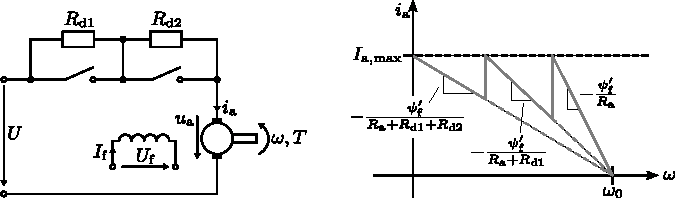
\includegraphics[scale=1.1]{fig/lec03/DC_machine_dropping_resistor.pdf}
				\caption{Operation with dropping resistor during start up to limit the armature voltage (adapted from J.~B\"ocker, \textit{Elektrische Antriebstechnik}, Paderborn University, 2020)}
				\label{fig:DC_machine_dropping_resistor}
		\end{figure}
\end{frame}

%%%%%%%%%%%%%%%%%%%%%%%%%%%%%%%%%%%%%%%%%%%%%%%%%%%%%%%%%%%%%
%% Operation constraints: separately excited DC machine %%
%%%%%%%%%%%%%%%%%%%%%%%%%%%%%%%%%%%%%%%%%%%%%%%%%%%%%%%%%%%%%
\begin{frame}
	\frametitle{Operation constraints: separately excited DC machine}
			Now we consider $U_\mathrm{a}$ being controllable (e.g., via buck converter), that is, we can also change $I_\mathrm{a}$. Nevertheless, the machine is still limited by the voltage and current constraint:
			\begin{equation}
				U_\mathrm{max} \leq U_\mathrm{a} = \frac{R_\mathrm{a}}{\psi_\mathrm{f}'} T + \omega \psi_\mathrm{f}', \qquad I_\mathrm{max} \leq I_\mathrm{a}.
				\label{eq:Operation_constraints_sep_DC_machine}
			\end{equation} \pause
			For sake of simplicity we only consider the first quadrant (cf. \figref{fig:machine_quadrants}), that is, positive torque and speed mode. \pause From \eqref{eq:Operation_constraints_sep_DC_machine} $T\leq \psi_\mathrm{f}' I_\mathrm{max}$ follows. \pause Also, the maximum speed is limited:
			\begin{equation}
				\omega \leq \frac{U_\mathrm{max}}{\psi_\mathrm{f}'} - \frac{R_\mathrm{a}}{\psi_\mathrm{f}'^2} T.
			\end{equation} \pause
			Hence, for a constant excitation $\psi_\mathrm{f}'$, the torque must be reduced starting at $\omega_1$ while $\omega_0$ represents the no-load speed where no torque can be generated anymore:
			\begin{equation}
				\omega_1 = \frac{U_\mathrm{max}}{\psi_\mathrm{f}'} - \frac{R_\mathrm{a}}{\psi_\mathrm{f}'} I_\mathrm{max}, \qquad \omega_0 = \frac{U_\mathrm{max}}{\psi_\mathrm{f}'}.
			\end{equation}
\end{frame}

%%%%%%%%%%%%%%%%%%%%%%%%%%%%%%%%%%%%%%%%%%%%%%%%%%%%%%%%%%%%%
%% Operation constraints: separately excited DC machine (cont.) %%
%%%%%%%%%%%%%%%%%%%%%%%%%%%%%%%%%%%%%%%%%%%%%%%%%%%%%%%%%%%%%
\begin{frame}
	\frametitle{Operation constraints: separately excited DC machine (cont.)}
	\begin{figure}
		\centering
		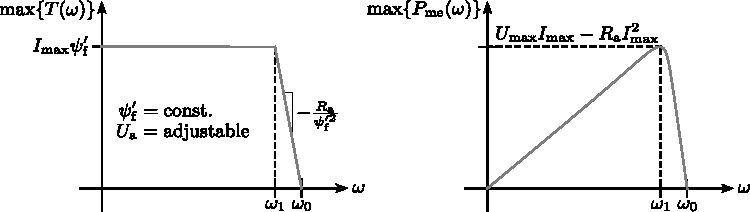
\includegraphics[scale=1.1]{fig/lec03/Sep_DC_machine_voltage_current_const.pdf}
		\caption{Maximum achievable torque and mechanical power for the separately excited DC machine with a fixed excitation $\psi_\mathrm{f}'$ but controllable armature voltage $U_\mathrm{a}$ and current $I_\mathrm{a}$}
		\label{fig:Sep_DC_machine_voltage_current_const}
\end{figure}
\end{frame}

%%%%%%%%%%%%%%%%%%%%%%%%%%%%%%%%%%%%%%%%%%%%%%%%%%%%%%%%%%%%%
%% Field weakening of the separately excited DC machine %%
%%%%%%%%%%%%%%%%%%%%%%%%%%%%%%%%%%%%%%%%%%%%%%%%%%%%%%%%%%%%%
\begin{frame}
	\frametitle{Field weakening of the separately excited DC machine}
			In the previous scenario, the no-load speed $\omega_0$ is limited by the maximum armature voltage $U_\mathrm{max}$. However, if the field winding current $I_\mathrm{f}$ is also controllable, the no-load speed can be increased by decreasing the excitation $\psi_\mathrm{f}'$ (so-called field weakening). \pause Consider an armature operation both at the voltage and current constraint:
			\begin{equation}
				U_\mathrm{max}  = R_\mathrm{a} I_\mathrm{max} + \omega \psi_\mathrm{f}'= R_\mathrm{a} I_\mathrm{max} + \omega L_\mathrm{f}' i_\mathrm{f}.
			\end{equation} \pause
			For $\omega > \omega_1$ the field weakening is applied by reducing $i_\mathrm{f}$ to stay exactly at the armature voltage constraint:
			\begin{equation}
				i_\mathrm{f} = \frac{1}{\omega}\frac{U_\mathrm{max} - R_\mathrm{a} I_\mathrm{max}}{L_\mathrm{f}'}.
			\end{equation} \pause
			Hence, we need to reduce the excitation with $1/\omega$ resulting in the torque and mechanical power
			\begin{equation}
				T = \frac{1}{\omega} \left(U_\mathrm{max}I_\mathrm{max} - R_\mathrm{a} I_\mathrm{max}^2\right), \qquad P_\mathrm{me} = U_\mathrm{max}I_\mathrm{max} - R_\mathrm{a} I_\mathrm{max}^2.
			\end{equation}
\end{frame}

%%%%%%%%%%%%%%%%%%%%%%%%%%%%%%%%%%%%%%%%%%%%%%%%%%%%%%%%%%%%%
%% Field weakening of the separately excited DC machine %%
%%%%%%%%%%%%%%%%%%%%%%%%%%%%%%%%%%%%%%%%%%%%%%%%%%%%%%%%%%%%%
\begin{frame}
	\frametitle{Field weakening of the separately excited DC machine (cont.)}
	\begin{figure}
		\centering
		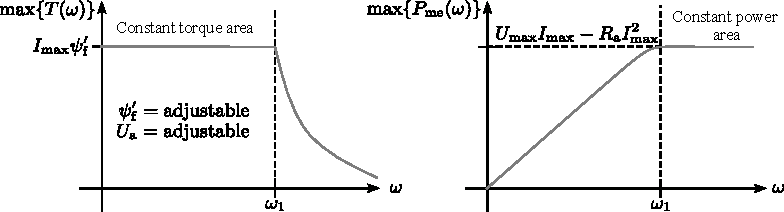
\includegraphics[scale=1.1]{fig/lec03/Sep_DC_machine_field_weakening.pdf}
		\caption{Maximum achievable torque and mechanical power for the separately excited DC machine with a variable excitation $\psi_\mathrm{f}'$ as well as controllable armature voltage $U_\mathrm{a}$ and current $I_\mathrm{a}$}
		\label{fig:Sep_DC_machine_field_weakening}
\end{figure}
\end{frame}

%%%%%%%%%%%%%%%%%%%%%%%%%%%%%%%%%%%%%%%%%%%%%%%%%%%%%%%%%%%%%
%% Steady-state behavior: shunt DC machine %%
%%%%%%%%%%%%%%%%%%%%%%%%%%%%%%%%%%%%%%%%%%%%%%%%%%%%%%%%%%%%%
\begin{frame}
	\frametitle{Steady-state behavior: shunt DC machine}
	\begin{columns}
		\begin{column}{0.55\textwidth}
		The shunt DC machine is characterized by:
	   \begin{equation}
		U = U_\mathrm{a}= U_\mathrm{f}, \qquad I = I_\mathrm{a} + I_\mathrm{f}.
	   \end{equation}
	   The steady-state currents are:
	   \begin{equation}
		\begin{split}
			I_\mathrm{f} &= \frac{U_\mathrm{f}}{R_\mathrm{f}},\\
			I_\mathrm{a} &= \frac{U_\mathrm{a} - \omega L_\mathrm{f}'I_\mathrm{f}}{R_\mathrm{a}} = \frac{1- L_\mathrm{f}'/R_\mathrm{f}\omega }{R_\mathrm{a}} U,\\
			I &= I_\mathrm{a} + I_\mathrm{f} = \left(\frac{1}{R_\mathrm{a}} + \frac{1}{R_\mathrm{f}} - \frac{L_\mathrm{f}'\omega}{R_\mathrm{a}R_\mathrm{f}}\right)U.
		\end{split}
		\end{equation}
		The resulting steady-state torque is:
		\begin{equation}
			T = L_\mathrm{f}' I_\mathrm{f} I_\mathrm{a} = L_\mathrm{f}'\frac{1- L_\mathrm{f}'/R_\mathrm{f}\omega }{R_\mathrm{a}R_\mathrm{f}}U^2.
		\end{equation}
\end{column}
\hfill
\begin{column}{0.45\textwidth}
	\begin{figure}
		\centering
		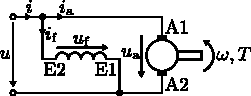
\includegraphics[scale=1.25]{fig/lec03/Shunt_DC_machine.pdf}
	\end{figure}
\end{column}
\end{columns}
\end{frame}

%%%%%%%%%%%%%%%%%%%%%%%%%%%%%%%%%%%%%%%%%%%%%%%%%%%%%%%%%%%%%
%% Steady-state behavior: series DC machine %%
%%%%%%%%%%%%%%%%%%%%%%%%%%%%%%%%%%%%%%%%%%%%%%%%%%%%%%%%%%%%%
\begin{frame}
	\frametitle{Steady-state behavior: series DC machine}
	\begin{columns}
		\begin{column}{0.55\textwidth}
		The series DC machine is characterized by:
	   \begin{equation}
		U = U_\mathrm{a} + U_\mathrm{f}, \qquad I = I_\mathrm{a} = I_\mathrm{f}.
		\label{eq:DC_series_machine_char}
	   \end{equation}
	   We can rewrite the terminal voltage as
	   \begin{equation}
		U = \left(R_\mathrm{a} + R_\mathrm{f}\right) I + \omega L_\mathrm{f}' I = R'(\omega) I 
	   \end{equation}
	   with the effective speed-dependent resistance
	   \begin{equation}
		R'(\omega) = R_\mathrm{a} + R_\mathrm{f} + \omega L_\mathrm{f}'.
	   \end{equation}
	   The steady-state torque is then
	   \begin{equation}
		T = L_\mathrm{f}' I^2 = L_\mathrm{f}'\left(\frac{U}{R'(\omega)}\right)^2.
		\label{eq:Torque_series_DC_machine}
	   \end{equation}
\end{column}
\hfill
\begin{column}{0.45\textwidth}
	\begin{figure}
		\centering
		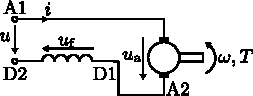
\includegraphics[scale=1.25]{fig/lec03/Series_DC_machine.pdf}
	\end{figure}
\end{column}
\end{columns}
\end{frame}

%%%%%%%%%%%%%%%%%%%%%%%%%%%%%%%%%%%%%%%%%%%%%%%%%%%%%%%%%%%%%
%% Steady-state behavior: series DC machine (cont.) %%
%%%%%%%%%%%%%%%%%%%%%%%%%%%%%%%%%%%%%%%%%%%%%%%%%%%%%%%%%%%%%
\begin{frame}
	\frametitle{Steady-state behavior: series DC machine (cont.)}
	\begin{columns}
		\begin{column}{0.55\textwidth}
		If the series DC machine is operated at the negative mechanical speed
		\begin{equation}
			\omega_\mathrm{r} = -\frac{R_\mathrm{a} + R_\mathrm{f}}{L_\mathrm{f}'},
	   \end{equation}
	   the current and the torque get (theoretically) infinite. This is due to the fact that the back EMF is exactly compensating the resistive voltage drop.

	   Moreover, for from \eqref{eq:Torque_series_DC_machine} we can observe that
	   \begin{equation}
		 T \rightarrow 0 \quad \Rightarrow \quad \omega \rightarrow \infty
	   \end{equation}
	   holds for any DC voltage $U \neq 0$. This is due to inherent, load-dependent flux weakening effect of the series DC machine.
\end{column}
\hfill
\begin{column}{0.45\textwidth}
	\begin{figure}
		\centering
		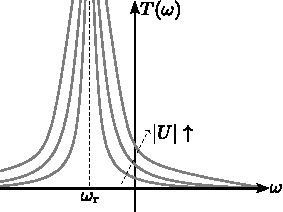
\includegraphics[scale=1.1]{fig/lec03/Series_DC_machine_torque_speed.pdf}
		\caption{Steady-state torque-speed characteristics for different DC voltage levels}
		\label{fig:Series_DC_machine_torque_speed}
\end{figure}
\end{column}
\end{columns}
\end{frame}

%%%%%%%%%%%%%%%%%%%%%%%%%%%%%%%%%%%%%%%%%%%%%%%%%%%%%%%%%%%%%
%% Universal motor: series DC machine with sinusoidal excitation %%
%%%%%%%%%%%%%%%%%%%%%%%%%%%%%%%%%%%%%%%%%%%%%%%%%%%%%%%%%%%%%
\begin{frame}
	\frametitle{Universal machine: series DC machine with sinusoidal excitation}
	\begin{columns}
		\begin{column}{0.55\textwidth}
		From \eqref{eq:Torque_series_DC_machine} it becomes clear that $T\sim I^2$ holds and, hence, the torque is independent of the sign of the current. Hence, the series DC machine can be also operated with an AC voltage supply (so-called universal machine).
		\\[1em] \pause 
		Consider the sinusoidal excitation 
		\begin{align*}
			u(t) &= \hat{u} \cos(\omega_\mathrm{el} t+ \varphi_{\mathrm{u}}) = \mathrm{Re}\left\{\hat{u} e^{\iu (\omega_\mathrm{el} t + \varphi_{\mathrm{u}})}\right\}\\ &= \mathrm{Re}\left\{\underline{U} e^{\iu \omega_\mathrm{el} t}\right\},	
		\end{align*} \pause
		which is represented by the complex phasor 
		\begin{equation}
			\underline{U} = U e ^{\iu \phi_{\mathrm{u}}} = \frac{1}{\sqrt{2}}\hat{u} e ^{\iu \varphi_{\mathrm{u}}}. 
		\end{equation}
\end{column}
\hfill \pause
\begin{column}{0.45\textwidth}
	\begin{figure}
		\centering
		\includegraphics[scale=1.05]{fig/lec03/Universal_machine_time_signals.pdf}
		\caption{Qualitative voltage, current and torque signals for an universal motor}
	\end{figure}
\end{column}
\end{columns}
\end{frame}

%%%%%%%%%%%%%%%%%%%%%%%%%%%%%%%%%%%%%%%%%%%%%%%%%%%%%%%%%%%%%
%% Universal motor: series DC machine with sinusoidal excitation (cont.) %%
%%%%%%%%%%%%%%%%%%%%%%%%%%%%%%%%%%%%%%%%%%%%%%%%%%%%%%%%%%%%%
\begin{frame}
	\frametitle{Universal machine: series DC machine with sinusoidal excitation (cont.)}
		From \eqref{eq:DC_machine_ODE_currents} and \eqref{eq:DC_series_machine_char} we can derive the complex voltage and current relations:
		\begin{equation}
			\underline{U} = R'(\omega)\underline{I} + \iu \omega_\mathrm{el} L \underline{I}
		\end{equation}
		with $L = L_\mathrm{f}+L_\mathrm{a}$. \pause The current phasor is
		\begin{equation}
			\underline{I} = \frac{\underline{U}}{R'(\omega) + \iu \omega_\mathrm{el} L}
		\end{equation} \pause
		resulting in the instantaneous current (setting $\varphi_{\mathrm{u}}=0$)
		\begin{align}
			i(t) &= \mathrm{Re}\left\{ \sqrt{2}\underline{I} e^{\iu\omega_\mathrm{el}t}\right\}=\sqrt{2}\mathrm{Re}\left\{ \frac{U\left(R'(\omega)-\iu\omega_\mathrm{el}L\right)}{R'(\omega)^2+\omega_\mathrm{el}^2L^2} e^{\iu\omega_\mathrm{el}t}\right\}\\
			& =\sqrt{2}\frac{U}{\sqrt{R'(\omega)^2+\omega_\mathrm{el}^2L^2}}\cos\left(\omega_\mathrm{el}(t-\frac{L}{R'(\omega)})\right).
		\end{align} 
\end{frame}

%%%%%%%%%%%%%%%%%%%%%%%%%%%%%%%%%%%%%%%%%%%%%%%%%%%%%%%%%%%%%
%% Universal motor: series DC machine with sinusoidal excitation (cont.) %%
%%%%%%%%%%%%%%%%%%%%%%%%%%%%%%%%%%%%%%%%%%%%%%%%%%%%%%%%%%%%%
\begin{frame}
	\frametitle{Universal machine: series DC machine with sinusoidal excitation (cont.)}
	\begin{columns}
		\begin{column}{0.55\textwidth}
		The resulting instantaneous torque is
		\begin{equation*}
		\begin{split}
			T(t) &= L_\mathrm{f}' i^2(t)\\
				 &= 2L_\mathrm{f}'\frac{U^2}{R'(\omega)^2+\omega_\mathrm{el}^2L^2}\cos\left(\omega_\mathrm{el}(t-\frac{L}{R'(\omega)})\right)^2\\
				 &= L_\mathrm{f}'\frac{U^2}{R'(\omega)^2+\omega_\mathrm{el}^2L^2}\left[1+\cos\left(2\omega_\mathrm{el}(t-\frac{L}{R'(\omega)})\right)\right].	
		\end{split}
	\end{equation*}
	\onslide<2->{
	The peak and average torque are
	\begin{equation}
		\begin{split}
		\hat{T} &= 2 L_\mathrm{f}'\frac{U^2}{R'(\omega)^2+\omega_\mathrm{el}^2L^2}= L_\mathrm{f}'\frac{\hat{u}^2}{R'(\omega)^2+\omega_\mathrm{el}^2L^2}, \\
		\overline{T} &= \frac{1}{2}\hat{T}.
	\end{split}
	\label{eq:Universal_motor_peak_avg_torque}
\end{equation}}
	\end{column}
\hfill
\begin{column}{0.45\textwidth}
	\begin{figure}
		\centering
		\includegraphics[scale=1.05]{fig/lec03/Universal_machine_time_signals.pdf}
	\end{figure}
\end{column}
\end{columns}
\end{frame}

%%%%%%%%%%%%%%%%%%%%%%%%%%%%%%%%%%%%%%%%%%%%%%%%%%%%%%%%%%%%%
%% Universal machine: series DC machine with sinusoidal excitation (cont.) %%
%%%%%%%%%%%%%%%%%%%%%%%%%%%%%%%%%%%%%%%%%%%%%%%%%%%%%%%%%%%%%
\begin{frame}
	\frametitle{Universal machine: series DC machine with sinusoidal excitation (cont.)}
	\begin{columns}
		\begin{column}{0.55\textwidth}
		\onslide<2->{
		Some remarks on the universal machine:}
		\begin{itemize}
			\item<2-> Only if the reactance $\omega_\mathrm{el}L$ impact on the voltage demand is negligible, the universal machine average torque at AC mode is identical to the series DC machine torque in DC mode applying the same effective voltage.
			\item<3-> Due to the AC field current, both the armature and stator should be based on a laminated iron core design to reduce iron losses.
			\item<4-> The peak armature and field currents are $\sqrt{2}$ times higher in the AC case than in DC operation. To prevent magnetic saturation, the iron paths must be designed larger than for an equivalent DC machine (i.e., leading to more volume and weight).
		\end{itemize}
\end{column}
\hfill
\begin{column}{0.45\textwidth}
	\begin{figure}
		\centering
		\includegraphics[scale=1.1]{fig/lec03/Universal_machine_torque_speed.pdf}
		\caption{Steady-state torque-speed characteristics for different AC voltage frequencies at a fixed voltage amplitude}
		\label{fig:Universal_machine_torque_speed}
\end{figure}
\end{column}
\end{columns}
\end{frame}

%%%%%%%%%%%%%%%%%%%%%%%%%%%%%%%%%%%%%%%%%%%%%%%%%%%%%%%%%%%%%
%% Commutation of the universal machine %%
%%%%%%%%%%%%%%%%%%%%%%%%%%%%%%%%%%%%%%%%%%%%%%%%%%%%%%%%%%%%%
\begin{frame}
	\frametitle{Commutation of the universal machine}
	\begin{columns}
		\begin{column}{0.65\textwidth}
		Assuming that the entire air gap field $\phi_\delta$ is linked by the commutation coil, the time-varying excitation field induces an additional spark voltage $u_\mathrm{sp}$ within the commutation coil:
		\begin{equation}
			u_\mathrm{sp} = -N_\mathrm{c} \frac{p}{a} \frac{\mathrm{d}\phi_\delta}{\mathrm{d}t}.
		\end{equation}
		\pause
		Due to the time-varying excitation current, we have $\phi_\delta(t) = \hat{\phi}_\delta\cos(\omega_\mathrm{el} t)$ and, hence,
		\begin{equation}
			u_\mathrm{sp} = N_\mathrm{c} \frac{p}{a} \omega_\mathrm{el} \hat{\phi}_\delta \sin(\omega_\mathrm{el} t).
			\label{eq:Induced_spark_voltage}
		\end{equation}
		\pause
		This additional induced spark voltage is shifted by (approx.) 90 degrees to the excitation field. Consequently, the interpole winding current is not in phase and does not compensate $u_\mathrm{sp}$.
\end{column}
\hfill
\begin{column}{0.35\textwidth}
	\onslide<1->
	\begin{figure}
		\centering
		\includegraphics[scale=1]{fig/lec03/Commutation_universal_machine.pdf}
		\caption{Simplified illustration of the induced voltage within the short-circuited commutation coil by the varying excitation field}
		\label{fig:Commutation_universal_machine}
\end{figure}
\end{column}
\end{columns}
\end{frame}

%%%%%%%%%%%%%%%%%%%%%%%%%%%%%%%%%%%%%%%%%%%%%%%%%%%%%%%%%%%%%
%% Commutation of the universal machine (cont.) %%
%%%%%%%%%%%%%%%%%%%%%%%%%%%%%%%%%%%%%%%%%%%%%%%%%%%%%%%%%%%%%
\begin{frame}
	\frametitle{Commutation of the universal machine (cont.)}
	\begin{columns}
		\begin{column}{0.65\textwidth}
		Assuming an ideal inductive behavior of the short-circuited coil, the induced spark voltage \eqref{eq:Induced_spark_voltage} leads to the current
		\begin{equation}
			i_\mathrm{sp} = -\frac{N_\mathrm{c} }{L_\mathrm{c} } \frac{p}{a} \hat{\phi}_\delta \cos(\omega_\mathrm{el} t).
		\end{equation}
		\pause
		This additional current will cause commutator sparking and, hence, the universal machine commutation process is more challenging than for a pure DC machine. 
		\pause
		\vspace{-0.25cm}
		\begin{varblock}{Conlusion on the universal machine}
			The drawbacks of the universal machine in terms of sizing and commutation sparking (leading to higher wear) are the reasons why this machine type is typical limited to low-cost applications (e.g., household appliances) nowadays. 
		\end{varblock}
\end{column}
\hfill
\begin{column}{0.35\textwidth}
	\onslide<1->
	\begin{figure}
		\centering
		\includegraphics[scale=1]{fig/lec03/Commutation_universal_machine.pdf}
\end{figure}
\end{column}
\end{columns}
\end{frame}